\documentclass[10pt,a4paper]{article}

\usepackage[utf8]{inputenc}


\usepackage{algpseudocode}
\usepackage{algorithmicx}
\usepackage{amsfonts}
\usepackage{amsmath}
\usepackage{amssymb}
\usepackage[spanish]{babel}
\usepackage[style=nature,intitle=true,sorting=none]{biblatex}
\usepackage{csquotes}
\usepackage{dsfont}
\usepackage{enumitem}
\usepackage{fancyhdr}
\usepackage{geometry}
\usepackage{graphicx}
\usepackage[hidelinks]{hyperref}
\usepackage{ifthen}
\usepackage[utf8]{inputenc}
\usepackage{multicol}
\usepackage{titling}
\usepackage{xcolor}
\usepackage{wrapfig}


\usepackage[style=nature,intitle=true,sorting=none]{biblatex}


\addbibresource{bibliography.bib}

\title{Organización del Computador II - Apuntes para final}
\author{Gianfranco Zamboni}

%%%% CONFIGURACIONES %%%%

%% La coma de los reales es un punto
\decimalpoint

%%% Tamaño de pagina
%\geometry{
%	includeheadfoot,
%	left=2.54cm,
%	bottom=1cm,
%	top=1cm,
%	right=2.54cm
%}

%\stul{0.1cm}{0.2ex}

%% HEADER Y FOOTER
\pagestyle{fancy}

\fancyhf{}

\fancyhead[LO]{\rightmark} % \thesection\ 
\fancyhead[RO]{\small{\thetitle}}
\fancyfoot[CO]{\thepage}
\renewcommand{\headrulewidth}{0.5pt}
\renewcommand{\footrulewidth}{0.5pt}
\setlength{\headsep}{1cm}
\setlength{\headheight}{13.07225pt}

\renewcommand{\baselinestretch}{1.2}  % line spacing

%% Links en indice 
\hypersetup{
	linktoc=all,     %set to all if you want both sections and subsections linked
	linkcolor=blue,  %choose some color if you want links to stand out
}

\newcommand{\red}[1]{{\color{red}#1}}  			% Rojo, duh (?)

\begin{document}
	\maketitle
	\tableofcontents

\newpage
\section{Introducción}

La \textbf{arquitectura de una computadora} es el conjunto de recursos accesibles para el programador que, por lo general, se mantienen a lo largo de los diferentes modelos de procesadores de esa arquitectura (puede evolucionar pero la tendencia es mantener compatibilidad hacia los modelos anteriores).

Diseñar una arquitectura implica diseñar las interfaces hardware/software para crear un sistema computacional que posea los requerimientos funcionales, de perfomance, consumo (de energía) y de costo (económico) adecuados para realizar determinadas tareas.

\begin{wrapfigure}{r}{0.5\textwidth}
	\centering
	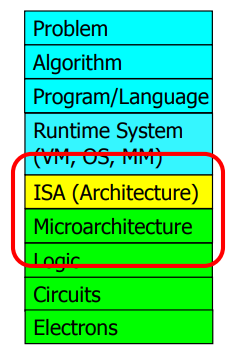
\includegraphics[width=0.25\textwidth]{imagenes/arquitectura}
	\caption{La computadora definida en niveles de abstracción}
	\label{fig:intro::arquitectura}
\end{wrapfigure}

Estas tareas son problemas que pasaron por varias transformaciones (desde su descripción en un lenguaje natural hasta convertirse en un programa) y deben ser ejecutadas por una computadora. La tarea del arquitecto consiste en diseñar el \textbf{Instruction Set Architecture} (ISA), un conjunto de instrucciones que usarán los programas compilados para decir al micropocesador que hacer. El ISA es implementado por un conjunto de estructuras de hardware conocidas como \textbf{microarquitectura}.

El ISA y la microarquitectura sientan las bases para que el diseño del procesador consiga el balance adecuado de los factores mencionados y pueda llevar a cabo ciertas tareas de la manera más optima posible. Habrá casos en los que daremos prioridad a un subconjunto de ellos en detrimento de otros (por ejemplo, podriamos elegir mejorar perfomance y aumentar el costo, o quitar performance para mejorar el consumo energético).

\subsection{Componentes del ISA}
El ISA es la especificación completa de la interfaz entre los programas y el hardware que debe llevar a cabo las operaciones. Entre otras cosas, especifica:

\subsubsection{Regitros}
\begin{itemize}
	\item \textbf{Registros:} Celdas de memoria dentro del cpu que son usadas para almacenar los datos necesarios para ejecutar una instrucción. Éstos, son visibles al programa y se clasifican según su uso: Acumuladores, De dirección ó De Proposito General.
	\item  \textbf{Instrucciones}: Tareas que pueden ser llevadas a cabo por la computadora. Cada una de ellas está compuesta por su \textbf{opcode} (que se espera que la computadora haga) y sus \textbf{operandos} (a que datos debe hacerlo). En una ISA podremos encontrar tres tipos de instrucciones:
	\begin{itemize}
		\item De \textbf{Operacion}: Procan datos.
		\item De \textbf{trasnporte}: Transportan información entre la memoria, los registros y los dispositivos de entrada salida.
		\item De \textbf{control (Branching)}: Modifican la secuencia de instrucciones a ser ejecutada, es decir, permiten ejecutar instrucciones que no están almacenadas secuencialmente.
	\end{itemize}
	
	Dependiendo que valores puedan modificar las instrucciones de operación, podremos clasificar las arquitecturas en: \textbf{Arquitecturas Load/Store} (solo pueden operar en registros) o \textbf{Arquitecturas memory/memory} (se pueden modificar los valores directamente en memoria)
	\item \textbf{Tipos de datos}: Representación que deben tener ciertos valores para poder ser interpretados por la microarquitectura.
	\item \textbf{Espacio de memoria}: La cantidad de bloques univocamente distinguibles en memoria y el tamaño de cada uno de estos bloques
	\item \textbf{Direccionamiento}: Los mecanismos usados por la computadora para saber donde están almacenados los datos. Puede ser:
	\begin{itemize}
		\item \textbf{Inmediato:} El operando está incluido en la instrucción.
		\item \textbf{Directo o absoluto:} El operando es la dirección de memoria donde se encuentra el valor a ser utilizado.
		\item \textbf{Indirecto:} El operando es una dirección de memoria donde se encuentra la dirección de memoria en la que está almacenado el valor deseado.
		\item \textbf{De desplazamiento:} La instrucción toma como operandos una dirección de memoria que se toma como \textbf{base} y un \textbf{offset}. La base es una dirección de memoria y el offset, un número que indica cuanto hay que desplazar la base para encontrar el valor deseado, es decir $dir = base + offset$
		\item \textbf{Indexado:} Lo mismo que el anterior, pero con el \textit{offset} guardado en un registro.
		\item \textbf{De Memoria Indirecta:} El operando es un registro en el que se encuentra guardada la dirección de memoria indirecta.
	\end{itemize}
	\item \textbf{I/O Interface}: Como comunicarse con los dispositivos de entrada/salida. Puede ser por medio de instrucciones especiales o mapeos de ciertas regiones memoria para uso de esos dispositivos.
	\item \textbf{Modos de privilegio:} Quien puede y quien no puede ejecutar ciertas instrucciones 
	\item \textbf{Manejo de expcepciones e interrupciones:} Qué debe suceder si una instrucción falla o cuando un dispositivo necesita usar el microprocesador.
	\item \textbf{Soporte de memoria virtual:} Si soporta o no el uso de \textbf{memoria virtual}, es decir, si cada programa tiene la ilusión de estar un espacio de memoria secuencial cuando en realidad el sistema operativo realiza el manejo de la memoria principal.
\end{itemize}

\subsubsection{Arquitectura de Von Neumann}\label{sec::Intro::ISA::Von_Neuman}
Como se vió en Organización del computador I, las mayoría de las ISA usadas actualmente usan el modelo de Von Neumann. Éste es un ciclo de cuatro etapas: 

\begin{enumerate}
	\item \textbf{Fecth:} Se utiliza un \textbf{program counter} para saber donde está almacenada la proxima instrucción a ser ejecutada. Y se carga desde la memoria.
	\item \textbf{Decode:} Se decodifica la instrucción fetcheada y se consiguen los operandos (literales y registros) correspondientes.
	\item \textbf{Execute:} En esta etapa se busca en memoria los datos requeridos (si es necesario) y se procesa los datos acorde a la instrucción.
	\item \textbf{Write Back:} Se almacenan los resultados obtenidos en el lugar indicado.
\end{enumerate}

\begin{figure}[ht]
	\centering
	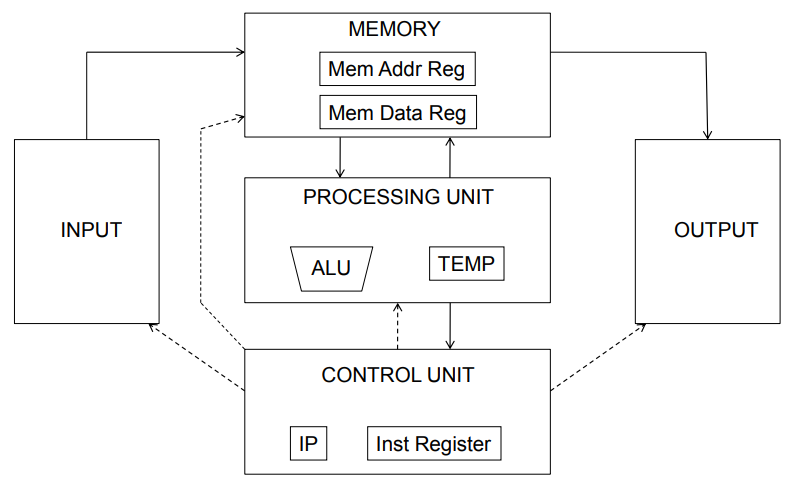
\includegraphics[width=0.4\textwidth]{imagenes/von-neuman-arquichtecture}
	\caption{Arquitectura de Von Newmman}
	\label{fig:intro:componentesIsa::vonsneumanarquichtecture}
\end{figure}
Cada instrucción es extraída de la memoria usando la dirección indicada por el \textbf{Instruction Pointer}. La unidad de control se encarga de indicar a la memoria si son necesarios otros valores para poder llevar a cabo su ejecución y, luego, pasa todo los datos a la unidad de procesamiento.

Si bien este es el ciclo que ``ve'' un programador, la implementación de las ISA (microarquitectura) usa estructuras de hardware más complejas que permiten acelerar la ejecución de cada fase.

\subsection{Microarquitectura}
La micoarquitectura es la implementación a nivel hardware de la ISA, es decir, es un conjunto de componentes electrónicos organizados de cierta manera para que respeten esas especificaciones.  Desde el punto de vista de la implementación (hardware), el ciclo es realizado por unidades de procesamiento que operan sobre los datos de acuerdo a ciertas señales. 

Cada instrucción es una señal que usa el procesador de instrucciones para decidir que conjunto de componentes electrónicos deben ser activados para poder llevar a cabo la operación deseada. Especificamente, las instrucciones indican: 

\begin{itemize}
	\item \textbf{Datapath:} Que elementos deben manejar y transformar los datos (unidades de procesamiento, de almacenamiento y estructuras de hardware que permiten el flujo de datos)
	\item \textbf{Control Logic:} Que elementos de hardware determinan las señales de control que indican al datapath lo que debe hacer con los datos.
\end{itemize}

En otras palabras, la microarquitectura comprende la tecnología utilizada para construir el hardware, la organización e interconexión de la memoria, el diseño de los bloques de CPU y la implementación de distintos mecanismos de procesamiento que no son visibles para el programador. 

%\subsection{Medidas de Performance}
%La escala y complejidad de los sistemas de software modernos, junto con las técnicas usadas por los diseñadores de hardware para mejorar el rendimiento de los dispositivos, ha logrado hacer que el rendimiento pueda depender de varios factores.
%
%\subsubsection{Response time}
%A veces, mediremos el rendimiento de una computadora en base a su tiempo de respuesta (\textbf{response time} o \textbf{execution time}) - el tiempo entre que pasa entre que una tarea empieza y termina -. Este tiempo se mide en segundos por programa y mide el tiempo total que toma completar una tarea, incluyendo accesos a memoria, operaciones del sistema, etc.
%
%En la práctica, la computadora es compartida por varios programas y los microprocesadores deben ejecutar varias tareas simultáneamente. En estos casos, deberemos tener en cuenta que la tarea que la tarea que se está evaluando, no está siendo ejecutada todo el tiempo por lo qué habrá que distinguir el tiempo que el procesador pasa ejecutando la tarea  \textbf{CPU Time} del tiempo en el que está procesando otros programas.
%
%Entonces, el tiempo de ejecución se define de la siguiente manera:
%
%$$Response~Time = \frac{Clock~Cycles~spent~on~task}{Clock~Rate}$$
%
%Donde \textit{Clock Cycle} son la cantidad de ciclos de reloj (ticks) que se utilizaron en la tarea y \textit{Clock Rate} es el tiempo que dura cada tick del reloj.


\newpage
\part{Subsistema de memoria}
\section{El sistema de memoria}
\subsection{Principio de vencidad o localidad}
\paragraph{Temporal Locality:} Una dirección de memoria que está siendo accedida actualmente tiene muy alta probabilidad de seguir siendo accedida en el futuro inmediato.

\paragraph{Spatial Locality:} Si actualmente se está accediendo a una dirección determinada de memoria, la probabilidad de que ésta y sus adyacentes sean accedidas en el futuro inmediato es muy alta.

La localidad de los programas surge naturalmente de su estructura. La mayoría contiene loops, osea que las instrucciones y los datos usados en ellos será accedido repetidamente lo que genera localidad temporal. Además, como son accedidas secuencialmente se tiene localidad espacial.

\subsection{Jerarquías de memoria}
Para aprovechar estos principios, se implementa la memoria de una computadora como una \textbf{jerarquía} que consiste en múltiples niveles de memoria con diferentes tamaños y velocidades. Mientras más rápida sean, más caras por bit son. El objetivo es presentar al usuario con tanta memoria como sea posible con la tecnología más barata proveyendo, al mismo tiempo, la velocidad de acceso provista por las memorias más rápidas.

En la actualidad hay tres tipos de tecnologías usadas para construir las distintas jerarquías. La memoria principal es implementada con DRAM (Dynamic Random Access Memory) mientras que los niveles más cercanos al procesador (caché) usan SRAM (Static Random Access Memory)  [Ver sección \ref{sec::Memoria::Tipos}].

\begin{figure}[ht]
	\centering
	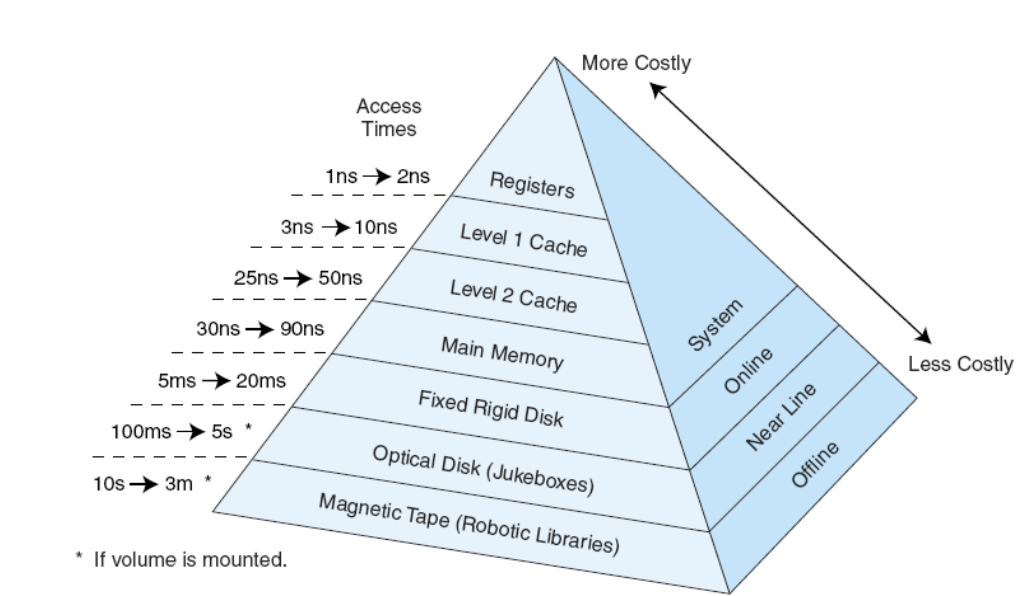
\includegraphics[width=1\textwidth]{imagenes/memory-heriarchy}
	\caption{Memory Hierarchy}
	\label{fig:memory-hierarchy}
\end{figure}

Sin importar el tamaño de la jerarquía, los datos son copiados solo entre dos niveles adyacentes. El nivel más alto - el más cercano al procesador - es más pequeño y rápido y usa tecnología más cara que el nivel más bajo.

\paragraph{Bloque:} La mínima unidad de información que puede estar presente en la jerarquía de dos niveles (la que está compuesta por las dos memorias que intercambian información).

\paragraph{Hit:} Se produce cuando la información pedida por el procesador se encuentra en algún bloque de la memoria que se está utilizando.

\paragraph{Miss:} Cuando la información debe ser buscada en el nivel inferior de la jerarquía.

\paragraph{Hit Rate:} La fracción de accesos a memoria encontrados en cada nivel de la jerarquía. A menudo es usado como medida de rendimiento de la misma.

\paragraph{Miss Rate: } 1 - hit rate (para cada nivel)

\paragraph{Hit time:} El tiempo que se tarda en acceder a un bloque en cada nivel de la jerarquía.

\paragraph{Miss penalty:} El tiempo requerido para fetchear un bloque desde el nivel inferior de la jerarquía (incluyendo tiempo de acceso, transmisión y copiado del bloque).

\newpage
\section{Tipos de memoria}\label{sec::Memoria::Tipos}
Hay dos tipos de memoria:


\begin{itemize}
	\item \textbf{No volátiles:} Son memorias capaces de retener la información almacenada cuando se les desconecta la alimentación. Son la tercera digievolución de las memorias \textbf{ROM} (Read Only Memory) que debían ser grabadas por el fabricante del chip y no eran modificables.
	
	De ROM pasaron a ser componentes programables que podían ser borrados con luz ultravioleta de una determinada longitud de onda. Y, luego, se convirtieron en las actuales memorias flash que pueden ser grabadas por algoritmos de escritura \textit{on the fly} por el usuario. El ejemplo más habitual son los discos de estado sólido de los equipos portátiles modernos.
	
	Se usan fundamentalmente para almacenar el programa de arranque de cualquier sistema.
	
	\item\textbf{Volátiles:} Conocidas como \textbf{RAM}, se caracterizan por que una vez interrumpida la alimentación eléctrica, la información que almacenaban se pierde.
	
	Estas memorias pueden almacenar mayor cantidad de información y modificarla en tiempo real a gran velocidad a comparación de las No Volátiles.
	
	Se clasifican de acuerdo con la tecnología y su diseño interno en:
	
	\begin{itemize}
		\item \textbf{Dinámicas (DRAM):} Almacenan la información en forma de una carga en un capacitor y la sostiene durante un breve lapso de tiempo con la ayuda de un transistor.
		
		Para guardar la información se activa el transistor que aplica el voltaje apropiado a la linea del bit. Una vez cargado el capacitor, se desactiva. 
		
		Después de un tiempo, la carga del capacitor (que se empieza a descargar) llega a un determinado threshold y en necesario volver a activar el transistor para cargar la información otra vez (si había un uno).
		
		Durante una operación de lectura, los capacitores de la celda seleccionada son activados y descargados completamente. En este caso, un amplificador detecta los valores leídos y aplica voltaje a las lineas de bits necesarias para volver a cargar
 		los capacitores necesarios. Esto aumenta el tiempo de acceso a la celda ya que no se puede liberar la operación hasta no haber repuesto el estado de carga de cada uno de ellos.
 		\item \textbf{Estáticas (SRAM):} Almacenan la información en un bi-estable Una celda se compone de seis transistores (por lo que tienen menos capacidad por componente que las dinámicas).
 		
 		Tres de los seis transistores están saturados (conducen la máxima corriente posible de forma permanente) y los otros tres están al corte (conducen una corriente prácticamente insignificante pero no nula). Esto genera un mayor consumo de energía por celda.
 		
 		La lectura es directa y no destructiva lo que se traduce en un tiempo de acceso bajo en comparación con las memorias dinámicas.
	\end{itemize}

\end{itemize}

\newpage
\section{Memoria Caché}
Los niveles de caché son bancos de SRAM de muy alta velocidad que contienen una copia de los datos e instrucciones que están en memoria principal. Deben ser lo suficientemente grandes para que el procesador resuelva la mayor cantidad posible de búsquedas de código y datos en memoria asegurando una alta performance y lo suficientemente pequeñas para no afectar el consumo ni el costo del sistema.

Para implementar estas memorias se debe agregar un controlador que se encarga de mantener la caché actualizada y de indicarle que datos debe mandar al procesador.

\subsection{Operación de lectura}
\begin{itemize}
	\item El procesador inicia un ciclo de lectura de memoria, envía la dirección necesaria al controlador de caché.
	\item El controlador busca la dirección en el directorio de la caché.
	\begin{itemize}
		\item Si hay un \textbf{hit}, busca el ítem en la memoria caché y lo envía al procesador.
		\item Si hay un \textbf{miss},  busca el ítem en el sistema de memoria y lo copia en la caché. Actualiza el directorio de la misma y después manda la data al procesador.
	\end{itemize}
\end{itemize}

\begin{figure}[ht]
	\centering
	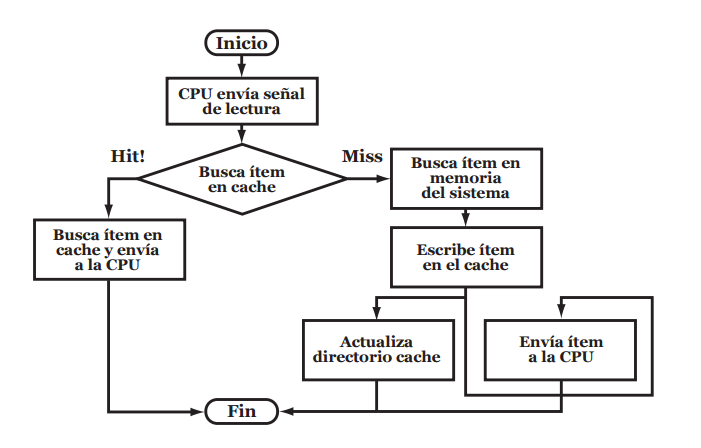
\includegraphics[width=1\textwidth]{imagenes/cache}
	\caption{Operación de lectura}
	\label{fig:reading-operation}
\end{figure}

\subsection{Organización de la caché}

\paragraph{Línea:} Elemento mínimo de palabra de datos dentro del caché. Corresponde a un múltiplo del tamaño de la palabra de datos de memoria. Esto nos permite copiar, en memoria, el ítem requerido y aquellos que lo rodean (principio de vecindad espacial).

\paragraph{Set:} Un conjunto que contiene $2^{ln}$ lineas de la caché.

\subsubsection{Mapeo directo}
Se divide, a la memoria en $2^j - 1$ paginas. Y cada página en $n$ bloques.

\begin{itemize}
	\item Los primeros $j$ bits de la dirección identifican la página a la que pertenece la línea.
	\item Los siguientes $n$, el set que les corresponde en la caché.
	\item Los $ln$ bits identifican la línea que le corresponde dentro del set
	\item y los últimos $b$ bits indican el índice de la palabra buscada dentro de la línea.
\end{itemize}

Para  buscar una dirección de memoria, en este tipo de caché:

\begin{itemize}
	\item Se busca el set en el que se encontraría esa dirección.
	\item Si el set tiene información válida, se corrobora que sea de la página de memoria a la que pertenece esa dirección.
	\begin{itemize}
		\item Si la página es correcta, entonces se accede al set en busca de la línea correspondiente y se vuelve el dato pedido
		\item Sino, se trae de memoria un bloque de tamaño del set y remplaza el set actual por ese.
	\end{itemize}
\end{itemize}
\begin{minipage}{\textwidth}
	\centering
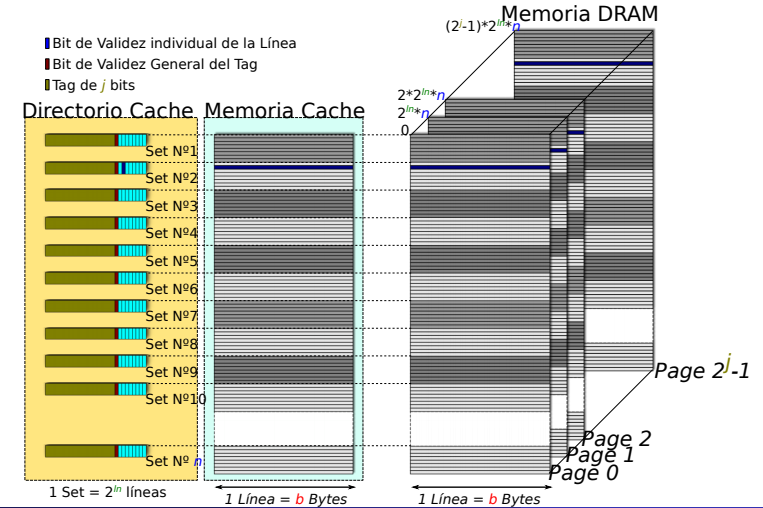
\includegraphics[width=\textwidth]{imagenes/cache-mapeo-directo}

Mapeo directo
	
\end{minipage}

\subsubsection{Totalmente asociativa}
Un bloque de memoria puede ser cargado en cualquier línea de la cache. Para determinar si un bloque se encuentra en la cache, se debe examinar el tag de todas las líneas para encontrar un match. Cuando la caché esta llena, se utiliza un algoritmo (generalmente least recently used - LRU)) para decidir que bloque remplazar.


Otros algoritmos de remplazo son FIFO (Firt In- First out, remplaza el bloque mas viejo) o LFU (Least frequently used, remplaza el bloque menos referenciado).

\subsubsection{Asociativa de dos vías}

Es una combinación de las dos anteriores. La cache se divide en dos y a un bloque le corresponde un set especifico. Sin embargo, dentro de ese set puede ser copiado en cualquiera de las dos mitades. Cuando hay que remplazar un bloque, se utiliza un LRU para decidir cual mitad usar.

\begin{minipage}{0.95\textwidth}
	\centering
		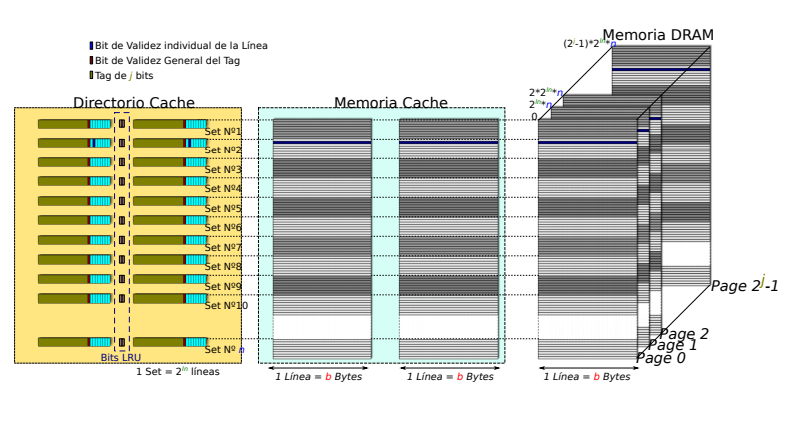
\includegraphics[width=0.95\textwidth]{imagenes/cache-asociativo-vias}
	
	Asociativo por 2 vías
	\label{fig:asociativo-mapping}
\end{minipage}

\subsection{Operación de escritura}

Cuando modificamos un valor, sería ideal que el cambio se vea reflejado tanto en la caché como en memoria principal. Si esto no pasa, entonces diremos que las memorias son inconsistentes/incoherentes.

Dependiendo del sistema (si hay una sola CPU o más de una) se utilizan distintas \textbf{políticas de escritura}. Decidir cuál de ellas usar constituye una de las decisiones más importantes en el diseño del sistema de memoria:

\begin{itemize}
	\item \textbf{Write through:} Cada vez que hay que hay que modificar una dirección, el procesador manda el dato tanto a memoria principal como al controlador de la caché y se realiza la escritura en ambas memorias. 
	
	Esto garantiza coherencia entre ambos datos de manera absoluta pero penaliza cada escritura con el tiempo de acceso a DRAM. Osea que la performance se degrada durante estas operaciones.
	
	\item \textbf{Write through buffered:} El procesador manda la data al controlador de caché que la actualiza y sigue ejecutando instrucciones y usando datos de la misma.
	
	El controlador dispone de un buffer de escritura que va almacenando estas modificaciones mientras se espera a que sean escritas a memoria. Cuando la escritura finaliza, se desencola y sigue con la próxima modificación.
	
 	Si el buffer está lleno cuando el procesador pide una escritura, entonces se debe parar la ejecución y esperar a que tenga una entrada libre. Si bien la ocurrencia de los stalls es reducida, estos siguen pasando.
 	
 	\item \textbf{Copy back / Write back:} Se modifican solo las líneas de la caché y se marcan como \textbf{dirty} (modificadas). El controlador escribe el bloque en memoria cuando debe ser remplazada por otro. 
 	
 	Este método mejora el performance cuando el procesador puede generar escrituras tan o más rápido de lo que puede escribir en memoria. Sin embargo, es mucho más difícil de implementar.
\end{itemize}

Si el procesador realiza un miss mientras el controlador caché está accediendo a la DRAM, deberá esperar a que la escritura termine para que su request sea atendido.

\subsubsection{Coherencia en sistemas multi-procesador (Snoop Bus)}


El bus es un conjunto de cables que conecta varios dispositivos, cada uno de los cuales puede observar cada transacción del mismo. Cuando un procesador emite un pedido a su caché, el controlador examina el estado de la misma y realiza las acciones adecuadas para completarlo. Esto puede generar transacciones para acceder a memoria.

\paragraph{SMP (Symetric Multiprocessors:)} Cada procesador posee una caché de primer nivel y todas ellas están conectadas al subsistema de memoria principal y dispositivos de E/S a través un único bus compartido.

\begin{figure}[ht]
	\centering
	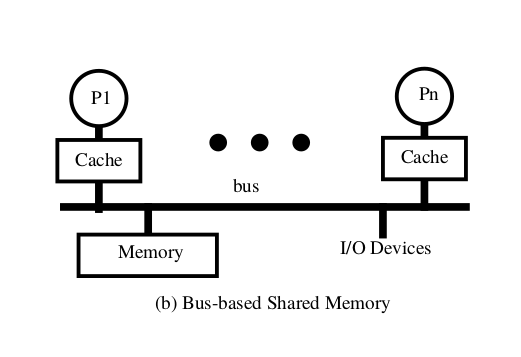
\includegraphics[width=0.5\textwidth]{imagenes/multiprocesor-caches}
	\caption{Bus de memoria compartido}
	\label{fig:busCompartido}
\end{figure}

Cuando un procesador modifica un bloque de memoria presente en su caché, se produce una incoherencia en las caches de los otros procesadores que tenían su propia copia del bloque. Esto sucede porque contienen un valor obsoleto en la dirección de memoria modificada por el primer procesador.

%\paragraph{Coherencia (en multiprocesadores):} Un sistema de memoria es coherente si es posible, para toda dirección, construir un orden serial de todas las operaciones que acceden a ella tal que:
%\begin{itemize}
%	\item Es consistente con los resultados de le ejecución.
%	\item Las operaciones emitidas por un procesador ocurren en el orden que fueron producidas por el mismo.
%	\item El valor devuelto por cada lectura es el valor escrito por la última operación de escritura en ese orden.
%\end{itemize}
%
%Está implícita, en esta definición, la propiedad de \textbf{serialización de escritura}. Ésta nos asegura que todos los procesadores ven todas las escrituras a una dirección en el mismo orden.

%\paragraph{Snooping bus:}
La coherencia se mantiene haciendo que cada controlador de caché espíe (snoop) el bus y monitoreé las transacciones. El controlador del bus funciona como arbitro para  decidir el orden en el que éstas son ejecutadas. Cuando una transacción es enviada por el bus, se envía la dirección a la que se está accediendo y el tipo de operación que se está realizando sobre ella.

Cada controlador de cache toma la dirección enviada por el bus y chequea si tiene una copia del bloque referenciado por la misma.

\begin{itemize}
	\item \textbf{Write-through:} Todas las escrituras se realizan directamente en la memoria principal. Todas las caches que tengan una copia del bloque modificado invalidan esa entrada. De esta forma, cuando el procesador necesite leer esa dirección, se tendrá que volver a cargar el bloque desde la memoria principal.
	
	El problema con este método es que se accede a memoria por cada operación de almacenamiento.
	
	\item  \textbf{Write-back:} Al momento es el método más utilizado ya que reduce drásticamente estos accesos. Sin embargo, no puede ser usado directamente en estos sistemas ya que no sería posible identificar donde está el último valor válido de una dirección. Por esta razón, se desarrollaron protocolos de coherencias (el más popular de ellos M.E.S.I) que nos permiten identificar la validez de nuestros datos.
\end{itemize}

\subsubsection{Protocolo MESI}
En este protocolo, un bloque de memoria en la caché puede estar en cuatro estados:

\begin{figure}[ht]
	\centering
	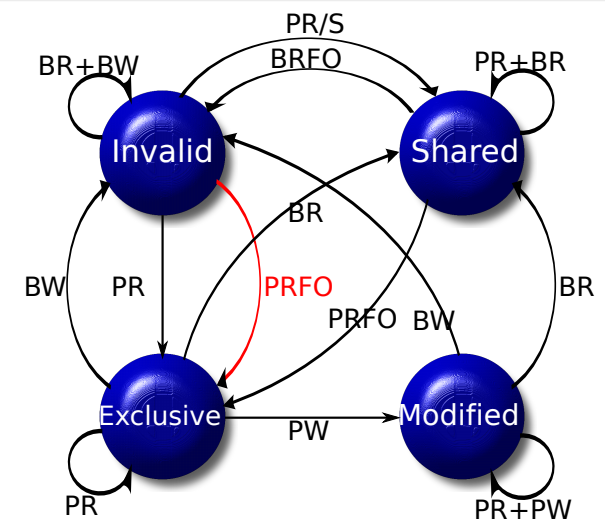
\includegraphics[width=0.5\textwidth]{imagenes/mesi-state-graph}
	\caption{Diagrama de estados de MESI. Cada nodo es un posible estado de un bloque de memoria. Supongmoas que vemos el proceso desde una caché. Las señales con prejifo ``P'' son las señales generadas por la misma (como lo ve la caché en la que estamos parados). Las señales con prefijo ``B'' es como actuán las demás cachés cuando ven la señal emitida por la caché en la que estamos parados. }
	\label{fig:mesiDiagram}
\end{figure}

\begin{itemize}
	\item \textbf{Modified (M):} Es la única copia valida. La memoria principal está desactualizada y ninguna otra caché tiene una copia valida del mismo bloque.
	\item \textbf{Exclusive (E):} Esa caché es la única que contiene una copia de ese bloque. Además, esa copia no está modificada.
	\item \textbf{Shared (S):} Está presente en esa caché sin ninguna modificación, la memoria principal está actualizada y puede haber otra caché que también lo tenga.
	\item \textbf{Invalid (I):} No está presente en la caché o contiene información desactualizada.
\end{itemize}

\paragraph{Lectura de un bloque:}
Supongamos que el procesador necesita leer un bloque de memoria, entonces produce una señal de tipo processor read (\textbf{PR}):
\begin{itemize}
	\item Si el bloque esta en caché (\textbf{Modified}, \textbf{Exclusive} o \textbf{Shared}), se resuelve el pedido.
	\item Si el bloque es \textbf{Invalid} entonces se genera un busRead (\textbf{BR}) y todas las cachés responden con una señal indicando si tienen o no una copia del valor pedido:
	\begin{itemize}
		\item Si no está en ninguna otra caché, se lo carga en modo \textbf{Exclusive} desde memoria principal.
		\item Si lo tiene alguna otra, se copia el bloque en modo \textbf{Shared} después de haber tomado las medidas necesarias para mantener la consistencia. Si la otra caché tiene el bloque:
		\begin{itemize}
			\item En modo \textbf{Exclusive}, se lo pasa a estado \textbf{Shared}.
			\item En modo \textbf{Modified}, se copian a memoria principal los cambios realizados y se lo pasa a \textbf{Shared}.
			\item En modo \textbf{Shared}, no se hace nada.
		\end{itemize}
	\end{itemize}
\end{itemize}

\paragraph{Escritura de un bloque:} Para escribir en un bloque, el procesador primero debe asegurarse que es el único con permisos de escritura, entonces:

\begin{itemize}
	\item Si el dato está en caché en modo \textbf{Modified} o \textbf{Exclusive}, genera un processor write (\textbf{PW}) y se modifica la caché. En el segundo caso, se pasa al estado \textbf{Modified}.
	\item Si el bloque está en modo \textbf{Invalid} ó \textbf{Shared}:
	\begin{itemize}
		\item Genera un Processor Request For Ownership (\textbf{PRFO}). Esto hace que su copia pase al estado \textbf{Exlusive} y la copia en todas las otras cachés pase a modo \textbf{Invalid}.
		\item Luego, genera el proccesor write (\textbf{PW}), realiza las modificaciones y pasa el bloque a \textbf{Modified}
	\end{itemize}
\end{itemize}

\begin{minipage}{0.95\textwidth}	\centering
	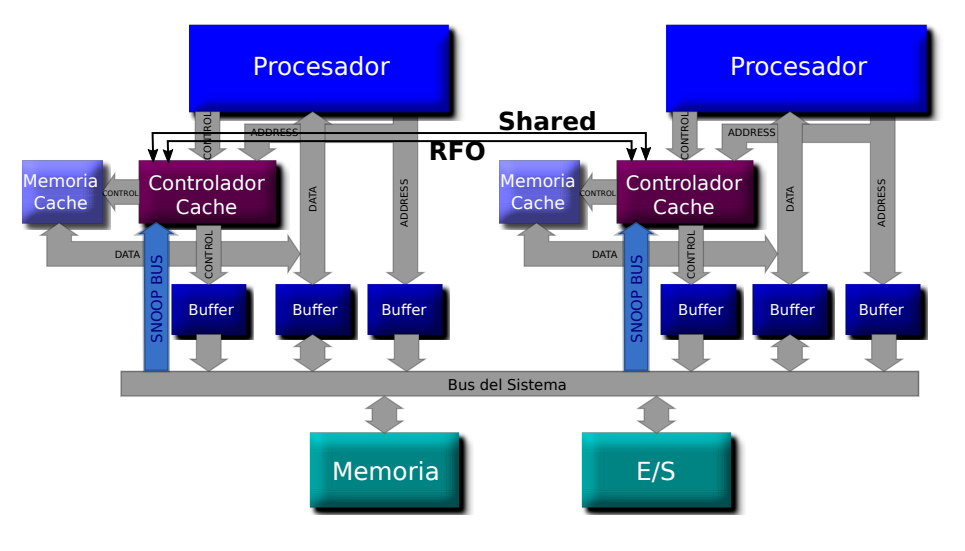
\includegraphics[width=0.95\textwidth]{imagenes/mesi-implementation}

	Implementación de MESI en un SMP
	\label{fig:mesiImplementation}
\end{minipage}

\subsubsection{Protocolo MESIF}
Este protocolo es una modificación de MESI desarrollada por Intel para arquitecturas de memoria no uniformes. Consiste de los 4 estados de MESI más un nuevo estado llamado \textbf{Forward} (F).

Este nuevo estado es una forma especializada de estado Shared e indica que esa caché fue designada para responder cualquier pedido de la línea correspondiente. El protocolo asegura que, si hay una caché que tiene la linea en estado \textbf{Shared} entonces hay por lo menos una caché que la tiene en estado \textbf{Forward}.

En los sitemas que emplean el protocolo MESI, el pedido de una linea que está en estado Shared en múltiples cachés es atendido de manera ineficiente. Puede ser respondido por la (lenta) memoria principal ó todas las cachés que la contienen pueden bombardear a la caché solicitante con respuestas redundantes.

En un sistema que hace uso de MESIF, el pedido de una linea será atendido solo por la caché que la contiene en estado \textbf{Forward}. Esto permite que la caché que hizo el request reciba una única copia a gran velocidad, evitando congestiones en el bus.

Como en el protocolo MESI, una caché puede descartar una línea en estado \textbf{Shared} ó \textbf{Forward} de manera unilateral, sin avisar al resto. Es posible que haya copias de una línea que estén estado \textbf{Shared} y ninguna esté en estado \textbf{Forward}. Para minimizar esta posibilidad, cuando una caché envía su copia de la línea, esta pasa a estado \textbf{Shared} y la caché que la recibe la guarda en estado \textbf{Forward}.

\newpage
\part{Instruction Level Parallelism}
\section{Pipelining}
El Pipeline es una técnica que permite superponer el procesamiento de múltiples instrucciones en una ejecución. Una vez que la primera instrucción fue fetcheada y pasa a la etapa de decodificación, se comienza a fetchear la siguiente instrucción. 

Bajo condiciones ideales y con un gran número de instrucciones, la mejora en velocidad de ejecución es directamente proporcional a la cantidad de etapas en el pipe. Es decir, un pipeline de 5 etapas, es aproximadamente 5 veces más rápido que el procesamiento secuencial.  

Si bien el pipelining reduce el tiempo de ejecución de un programa, debemos notar que no lo hace modificando el tiempo que se tarda en procesar una instrucción (\textbf{latency / latencia}) sino que aumenta la cantidad de instrucciones que se procesan por unidad de tiempo (\textbf{throughput}).
\begin{figure}[h]
	\centering
	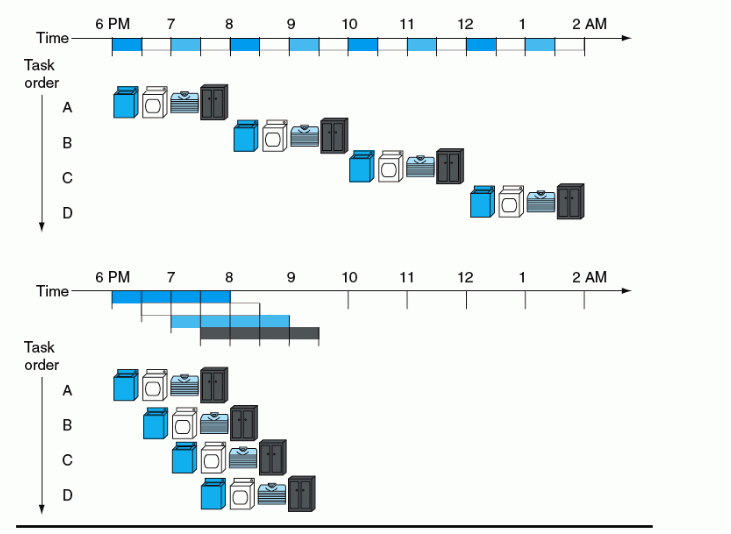
\includegraphics[width=0.5\linewidth]{imagenes/pipelining}
	\caption{Analogía de la lavandería: 4 personas tienen que lavar, secar, doblar y guardar su ropa sucia. Solo disponemos de una lavadora, una secadora, un ``doblador'' y un ropero. Si cada parte del proceso toma 30 minutos, y lo realizamos de manera secuencial, completarlo para las 4 personas tomaría ocho horas, mientras que si lo hacemos con un pipeline el tiempo se reduce a tres horas y media.}
	\label{fig:pipelining}
\end{figure}

Para facilitar una implementación efectiva del pipeline, el set de instrucciones propuesto debe permitir que todas las etapas tarden el mismo tiempo en ser ejecutadas. Esto implica que hay que tener ciertas consideraciones al momento de diseñarlo:

\begin{itemize}
	\item Todas las instrucciones deben tener la misma longitud (en la arquitectura IA-32, donde las instrucciones tienen longitud variada, esto se logra descomponiendo cada instrucción en micro-operaciones de longitud fija y a estas micro-operaciones se les aplica el pipelining).
	\item Todas las instrucciones deben tener la misma estructura, es decir, la cantidad de parámetros y la ubicación dentro de la instrucción que los explicita deben ser las mismas (o lo más parecidas posibles). 
	\item Los operandos deben estar alineados en memoria. Esto es, las direcciones de memoria que ocupan deben ser múltiplo del tamaño de las palabras usadas para que los datos puedan ser transferidos en una única etapa del pipeline.
\end{itemize}

\subsection{Pipeline Hazards}
Hay situaciones en las que una instrucción no puede ser ejecutada en el siguiente ciclo de reloj debido a algún obstáculo (\textbf{hazards}). Estos eventos pueden llegar a detener el flujo del pipeline (\textbf{pipeline stall}) y generar una demora en el procesamiento de las instrucciones. A continuación veremos los tres tipos de obstáculos que se pueden dar:

\begin{itemize}
	\item \textbf{Estructurales (Structural Hazards):} El hardware no soporta la combinación de instrucciones que queremos ejecutar en el mismo ciclo de reloj. Por ejemplo, si una instrucción debe acceder a memoria mientras otra debe realizar un fetch en la misma memoria. En este caso, las dos instrucciones deben utilizar los mismos recursos y debería dársele prioridad a la primera instrucción dejando a la segunda en espera.
	
	Para resolver esto debería agregarse hardware (como buffers, caches, etc).
	\item \textbf{De datos (Data Hazards):} Hay una instrucción en el pipeline que depende de los resultados de otra instrucción (también en el pipeline) y debe esperar a que ésta se complete para poder terminar. Esto puede bloquear el pipe durante varios ciclos de reloj ya que se debe procesar completamente la primer instrucción. 
	
	Para minimizar el impacto de este obstáculo, por lo general, se agrega extra hardware que permite conseguir el valor deseado apenas sea calculado (cuando termina la etapa de ejecución) directamente de los componentes internos para no tener que esperar a que sea guardado en memoria (esta técnica se llama \textbf{forwarding} o \textbf{bypassing}).
	
	\item \textbf{De control (Control or Branch Hazards):} La instrucción que se fetcheó no es la que debe ejecutarse en este ciclo de reloj. Cuando aparece una instrucción de control es fetcheada, el pipeline no puede saber cual es la próxima instrucción que debe ser ejecutada ya que esto depende del resultado de la instrucción actual.
	
	Una posible solución es parar apenas se haga el fetch del condicional y esperar hasta obtener sus resultado. Otra, es realizar predicciones (\textbf{branch prediction}) y ejecutar las instrucciones con más probabilidad de ser ejecutadas. En este último caso, el pipeline procede sin demoras si la predicción fue correcta sino debe eliminar las instrucciones procesadas y volver a comenzar desde el lugar correcto.
\end{itemize}

\newpage
\section{Branch Prediction}\label{sec::branchPrediction}

\paragraph{Branching:} Cuando se fetchea una instrucción condicional, se genera una ramificación en el código. Hay dos caminos posibles por el que puede seguir la ejecución y el camino que se debe ejecutar lo decide el resultado de la instrucción fetcheada. 

\paragraph{Untaken Branch:} Se dice cuando el camino tomado es el que ejecuta la instrucción que le sigue al condicional dentro del programa.

\paragraph{Taken Branch:} Cuando se ejecuta la instrucción que se encuentra en la dirección del salto de la instrucción condicional.

\paragraph{Branch penalty:} Cuando se fetchea la instrucción incorrecta, debe descartarse todo lo que estaba pre-procesado hasta ese momento. El pipeline se vacía y deben transcurrir $n-1$ ciclos de clock hasta el próximo resultado ($n = $ cantidad de etapas del pipeline).

\subsection{Predicciones estáticas}
\begin{itemize}
	\item \textbf{Assume Branch Not Taken:}  Se fetchea la siguiente instrucción secuencial del programa. Si el salto no se realiza entonces la ejecución del pipe continúa sin problemas. Si el salto se realiza, se aplica el branch penalty.
	\item \textbf{Assume Branch Taken}: Análogo al anterior pero se fetchea la instrucción en la dirección de memoria apuntada por el salto.
	\item \textbf{Predict by Opcode}: Se asume que el salto va a ser tomado o no dependiendo de la instrucción a ser ejecutada.
\end{itemize}

Este tipo de predicciones funcionan bien para piplines simples. Sin embargo, la penalidad de descartar instrucciones y el tiempo que se tarda en restaurar el sistema aumenta acorde a la complejidad del mismo. Las predicciones dinámicas intentan disminuir este problema manteniendo estadísticas de uso y modificando la decisiones tomadas a medida que se realiza la ejecución.

\subsection{Predicciones dinámicas}

\begin{itemize}
	\item\textbf{Branch Prediction Buffer}: Se mantiene una tabla indexada por la dirección de memoria de la instrucción del salto y 2 bits que indican si los últimos dos saltos hacia esa instrucción fueron tomados o no.
	
	\begin{figure}[ht]
		\centering
		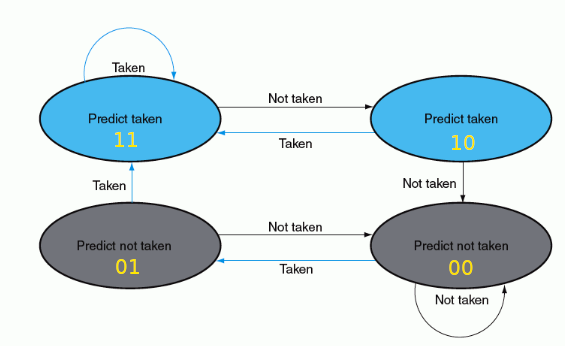
\includegraphics[width=0.7\linewidth]{imagenes/2bit-buffer-prediction}
		\caption{Maquinas de estados de predicción para un buffer de 2 bits}
		\label{fig:2bit-buffer-prediction}
	\end{figure}

	Las primeras implementaciones de esta técnica hacían uso de un único bit que se remplazaba cada vez que la predicción fallaba. En ciertos casos, la eficiencia de este método no era satisfactoria llegando a fallar completamente en otros (por ejemplo, si los saltos termina formando una secuencia intercalada de Taken y Not taken).
	
	\item \textbf{Branch Target Buffer (BTB)}: Es una caché en la que se almacena, en cada entrada, la dirección de la instrucción de control y la dirección de la instrucción que fue ejecutada después de resolver el branching.
	
	Cuando se fetchea una instrucción de control, se accede a esta caché usando el valor del program counter.
	\begin{itemize}
		\item Si el valor no está en el buffer, entonces se asume \textit{taken}.
		\begin{itemize}
			\item Si el resultado es \textit{Non-Taken} se acepta el delay en el pipeline y no se almacena nada en el BTB.
			\item Si el resultado es \textit{taken}, se ingresa el valor al BTB.
		\end{itemize}
		\item Si el valor se encuentra en el BTB, se aplica el campo de dirección de target almacenado.
		\begin{itemize}
			\item si el resultado es \textit{taken} no hay penalidad. No se guarda en el BTB ningún nuevo valor ya que el que está almacenado es el que nos sirve.
			\item Si el resultado es \textit{Non-taken}, guarda el nuevo valor en el BTB, luego de la penalidad correspondiente en el pipeline. 
		\end{itemize}
	\end{itemize}
\end{itemize}

\newpage
\section{Procesadores Superscalares}
Son procesadores que explotan la ejecución paralela de instrucciones para mejorar el rendimiento. Agrega más pipelines a la ejecución, lo que permite incrementar aún más la cantidad de instrucciones procesadas por ciclo de reloj.

Un problema es que los obstáculos estructurales quedan más expuestos. Cada etapa, ademas de lidiar con los data hazards de su propio pipeline, debe lidiar también con las mismas etapas del otro pipeline. 

Este tipo de procesadores analizan los binarios secuenciales de los programas y lo paralelizan eliminando esencialidad innecesaria. Por esta razón, los programas binarios deben ser vistos más como una especificación de lo que debe hacerse y no como lo que realmente sucede.

Más precisamente, un procesador superescalar implementa:

\begin{enumerate}
	\item Estrategias de fetch que permiten fetchear múltiples instrucciones mediante la predicción de resultados y saltos.
	\item Métodos para determinar dependencias de registros y mecanismos para comunicar esos valores cuando sea necesario durante la ejecución.
	\item Métodos para iniciar, o resolver, múltiples instrucciones en paralelo.
	\item Recursos para la ejecución en paralelo de varias instrucciones, incluyendo múltiples unidades funcionales de pipelines y jerarquías de memorias capaces de atender simultáneamente múltiples referencias a memoria.
	\item Métodos para manejar datos a través de instrucciones de lectura/escritura e interfaces de memoria que tengan en cuenta el comportamiento dinámico (y muchas veces impredecibles) de las jerarquías diseñadas.
	\item Métodos para actualizar los estados del proceso en el orden correcto (para mantener la apariencia de la ejecución en orden secuencial).
\end{enumerate}

\subsection{Dependencias de instrucciones}\label{sec:instructionLevelParalelism:dependenciaDeInstrucciones}
Por lo general, se interpreta el binario de un programa como un conjunto de bloques compuestos de instrucciones contiguas. Una vez que se fetchea un bloque, se sabe que todas sus instrucciones van a ser ejecutadas eventualmente. Cuando esto suceda, diremos que el bloque es iniciado en una \textbf{ventana de ejecución}.

Una vez que las instrucciones entran en esta ventana, son ejecutadas en paralelo teniendo en cuenta sus dependencias que pueden ser de control o datos. Las de control son generadas por condicionales y pueden ser resueltas/optimizadas con predicciones (Sección \ref{sec::branchPrediction}). 

Las \textbf{dependencias de datos} se da entre instrucciones que referencian el mismo espacio de memoria. En estos casos, si las instrucciones no se ejecutan en el orden correcto, puede haber errores en las operaciones. Pueden ser Verdaderas o Artificiales
\begin{itemize}
	\item \textbf{Dependencias verdaderas:} Cuando una instrucción debe leer un valor que todavía no fue generado por una instrucción previa (\textbf{Read after write hazard}).
	\item \textbf{Dependecias artificiales:} Resultan de instrucciones que deben escribir un nuevo valor en una posición de memoria pero debe esperar a que las instrucciones previas utilicen el valor actual (\textbf{Write after Read hazard}) o cuando varias instrucciones deben escribir la misma posición de memoria (\textbf{Write after Write hazard}).
	
	Estas dependencias son producidas por código no optimizado, por escasez de registros disponibles, por el deseo de economizar el uso de la memoria principal o por ciclos donde una instrucción puede colisionar consigo misma.
	
\end{itemize}


\subsection{Fetching and Decode}\label{ilp::superscalars::fetchDecode}
En los procesadores superescalares, una caché de instrucciones se usa para reducir la latencia y incrementar el ancho de banda del fetching. Esta caché está organizada en bloques o lineas que contienen varias instrucciones consecutivas y almacena el tipo de cada una de ellas (si es de control, de operación, de lectura de memoria, etc). 

El program counter se utiliza para determinar la posición de una instrucción en la caché.

\begin{itemize}
	\item Si se produce un hit, se fetchea el bloque de instrucciones y se suma al program counter el tamaño del bloque fetcheado.
	\item Si hay un miss, el caché pide la instrucción buscada en memoria y la copia.
	\item Se identifica el tipo de cada instrucción. Si alguna es de control, se realizan las predicciones usando alguno de los métodos mencionado en en la sección \ref{sec::branchPrediction}.
	\item Las instrucciones son decodificadas en  \textbf{tuplas de ejecución} que contienen la operación a ser ejecutada, las identidades de los elementos donde se encuentran los parámetros de entrada y donde deben guardase los resultados. 
	
	En el programa estático, las instrucciones utilizan los registros \textbf{lógicos} (los de la arquitectura). Por esta razón, cuando son decodificadas, se mapean (o renombran) a un registro físico y las dependencias artificiales se resuelven indicando a las instrucciones involucradas que usen distintos registros físicos (\textbf{Algoritmo de tomasulo}, sección \ref{ilp::tomasulo}).

	\item Una vez que todas las instrucciones asociadas a un registro físico son completadas (modifican el estado visible), se libera el registro para que pueda ser usado por otro bloque de instrucciones. 		
\end{itemize}

\subsection{Scoreboarding}
Cuando una instrucción es decodificada, se loguea en un archivo de registros llamado \textbf{scoreboard}. Éste se encarga de commitear, mandar a ejecutar y detectar dependencias. Cuando detecta que las instrucciones pueden leer sus operandos las manda a ejecutar. Si decide que no puede hacer esto, monitorea cada cambio del hardware hasta que los operandos necesarios estén disponibles.
Además, controla cuando una instrucción puede escribir sus resultados en el registro correspondiente. De esta manera, la detección de hazards y su resolución es centralizada en el scoreboard. 

Durante la ejecución, cada instrucción pasa por cuatro etapas:

\begin{enumerate}
	\item \textbf{Issue:} Si hay una unidad funcional libre para la instrucción y ninguna otra instrucción activa necesita escribir en el registro destino, el scoreboard la envía a esta unidad y actualiza su estado interno. Si hubiese otra instrucción que necesita del mismo registro, entonces se bloquea (\textit{stall}) hasta que todos los obstáculos hayan sido resueltos.
	
	Cuando esta etapa se bloquea \textit{stall}, el buffer de Fetching también entra en este estado cuando se llena.
	
	\item \textbf{Lectura de operandos:} Un operando se encuentra disponible si ninguna instrucción activa emitida anteriormente necesita escribirlo. Cuando los operandos fuentes están habilitados, el scoreboard le dice a la unidad funcional que proceda a leerlos desde los registros y comience la ejecución. De esta forma se  evitan los RAW hazards que, como se resuelven dinámicamente, permiten que las instrucciones sean ejecutadas fuera de orden.
	
	\item\textbf{Ejecución:} Las unidades funcionales comienzan la ejecución después de haber recibidos todos los operandos. Cuando el resultado está listo, lo notifica al scoreboard.
	
	\item\textbf{Escritura de resultado:} Una vez que el scoreboard recibe la notificación, chequea por WAR hazards. Si los encuentra, bloquea la escritura de la instrucción hasta que estos son resueltos.
\end{enumerate}

\paragraph{Desventajas de este método}
\begin{itemize}
	\item No puede aprovechar el forwarding de datos porque considera que un operando solo está listo cuando fue escrito en registro.
	\item El scoreboard controla el progreso de una instrucción comunicándose con las unidades funcionales. Al haber un numero limitado de buses de operandos y resultados, debe asegurarse que el número de unidades funcionales habilitadas para proceder no excedan estos recursos.
\end{itemize}
\subsection{Tomasulo}\label{ilp::tomasulo}
El algoritmo de Tomasulo crea un scheduling dinámico que permite ejecutar instrucciones fuera de orden y habilita el uso de múltiples unidades de ejecución. Para lograr esto necesita:
\begin{itemize}
	\item Mantener un ``link'' entre el productor de un dato con su(s) consumidor(es).
	\item Mantener las instrucciones en espera hasta que estén listas para ejecución.
	\item Saber cuando sus operandos están listos (``Ready'').
	\item Despachar (``dispatch'') cada una de ellas a su Unidad Funcional correspondiente ni bien todos sus operandos estén listos.
\end{itemize}

\paragraph{Register Renaming:} El primer ítem se logra asignando a cada registro un alias. Para eliminar los WAR y WAW hazards, se utiliza una tabla llamada \textbf{Register Alias Table} que asocia un tag con cada operando de una operación.

\paragraph{Register Station (RS):} Una vez realizado el renombre se le asigna, a la instrucción, un RS. Un RS es un subsistema de hardware compuesto de bancos de registros internos que se encarga de mantener las instrucciones en espera hasta que estén listas para ser ejecutadas. Éste chequea constantemente por la disponibilidad de los operandos de la instrucción. Para cada uno de ellos cuyo valor no esté disponible, el RS, guarda el \textit{tag} que se le asignó en el paso anterior.

Cada vez que una unidad de ejecución pone disponible un operando, transmite el \textbf{tag} asociado al mismo junto con su valor a todas las RS. Cuando una instrucción tiene todos sus operandos disponible, el RS espera a que la unidad funcional asociada a ella esté libre y luego la despacha.

\paragraph{Common Data Bus}: Es un datapath que cruza la salida de las unidades funcionales y atraviesa las RS, los Floating Point Buffers, los Floating Points Registers y el Floating Point Operations Stack. Se usa para realizar el broadcast de los resultados al finalizar cada operación.

\paragraph{Pseudocodigo:}
Cada Registro contiene un tag que indica el último escritor en el registro.

\begin{algorithmic}
	\If{RS tiene recursos disponibles antes del renaming}
	\State{Se inserta en la RS la instrucción y los opernados renombrados (valor fuente / tag)}
	\State{Se renombra si y solo si la RS tiene recursos disponibles.}
	\Else
	\State{stall}
	\EndIf
	\While{esté en la RS, cada instrucción debe}
	\State{Mirar el tráfico por el \textbf{Common Data Bus (CDB)} en busca de \textbf{tags} que correspondan a sus Operandos fuente.}
	\State{Cuando se detecta un \textbf{tag}, se graba el valor de la fuente y se mantiene en RS.}
	\State{Cuando ambos operandos están disponibles, la instrucciónn se marca \textbf{Ready} para ser despachada}
	\If{Unidad Funcional disponible}
	\State{Se depscacha la instrucción a esa unidad funcional}
	\EndIf
	\If{Finalizada la ejecución de la instrucción}
	\State{La unidad funcional pone el valor correspondiente al \textbf{tag} en el \textbf{CD} (\textbf{tag broadcast})}
	\If{El archivo de registros está conectado al CDB}
	\If{tag del Archivo de Registro $==$ tag broadcast}
	\State{Registro = valor broadcast}
	\State{bit de validez = '1'}
	\State{Recupera \textbf{tag} renombrado}
	\State{No queda copia válida del tag en el sistema}
	\EndIf
	\EndIf
	\EndIf
	\EndWhile
\end{algorithmic}


\subsection{Ejecución de instrucciones}
\subsubsection{Interrupciones}
Existen dos tipos de interrupciones:
\begin{itemize}
	\item \textbf{Excepciones} (o trampas): Se generan cuando se produce un error durante la ejecución o el fetching de ciertas instrucciones. Por ejemplo, opcodes ilegales, errores numéricos o page faults.
	\item \textbf{Interrupciones externas}: Son causadas por instrucciones específicas y dispositivos externos qué están ejecutando algún proceso. Por ejemplo las interrupciones generadas por los dispositivos de entrada/salida (mouse, teclados, pantallas), timers, etc.
\end{itemize}

Cuando ocurre una interrupción, el software o el hardware (o una combinación de ambos) guardan el estado del proceso interrumpido. Este estado consiste, generalmente, del program counter, los registros y la memoria.

\paragraph{Interrupción precisa:} Una interrupción es precisa si el estado guardado es consistente con la arquitectura secuencial del modelo. Osea se debe cumplir que:
\begin{enumerate}
	\item Todas las instrucciones previas a la indicada por el program counter deben haber sido ejecutadas y deben haber modificado el estado del proceso correctamente.
	\item Ninguna de las instrucciones siguientes a la indicada por el program counter debe haber sido ejecutadas ni deben haber modificado el estado del proceso.
	\item Si la interrupción es causada por una excepción en una instrucción del programa, entonces el program counter guardado debe apuntar a la instrucción interrumpida.
\end{enumerate}

Si el estado guardado es inconsistente con el modelo de arquitectura secuencial y no satisface estas condiciones entonces la interrupción es \textbf{imprecisa}. 

\subsubsection{In-Order Instruction Completion}
Las instrucciones modifican el estado del proceso solo cuando se sabe que todas las instrucciones previas están libres de excepciones. Para asegurar esto se utiliza un registro llamado ``result shift register'' que contiene una tabla de $n$  entradas ($n$ la longitud del pipeline más largo). Una instrucción que toma $i$ ciclos de reloj, reserva la $i$-ésima entrada de la tabla y en cada ciclo se la desplaza una posición hacia abajo.
\begin{figure}[ht]
	\centering
	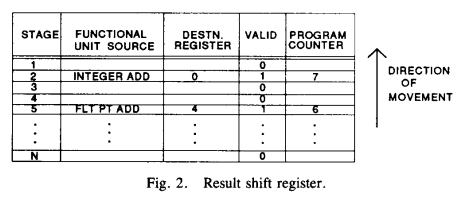
\includegraphics[width=0.5\linewidth]{imagenes/shift-register}
	\caption{Result Shift Register}
	\label{fig:shiftregister}
\end{figure}

Si la $i$-ésima entrada contiene información valida entonces se pausa la instrucción. En el próximo ciclo, se re chequea si la entrada está libre y se realiza el movimiento.

Para evitar que una instrucción más corta se complete antes que otra de mayor longitud (cuando este es el orden deseado) se rellenan con información invalida todas las entradas anteriores que no fueron reservadas. De esta forma, la nueva instrucción es pausada hasta el próximo ciclo de reloj.

\subsubsection{Reorder-Buffer}
La principal desventaja del método anterior es que instrucciones rápidas serán retenidas a pesar de no tener dependencias.

Para resolver este problema se agrega un \textbf{reorder buffer} que indica el orden en el que las instrucciones deben modificar el estado visible. Entonces se permite que las instrucciones terminen en cualquier orden pero se les asigna un tag que cumple con el objetivo mencionado. Cuando son completadas, se las almacena en la entrada indicada (por el tag) del buffer.

\begin{figure}[ht]
	\centering
	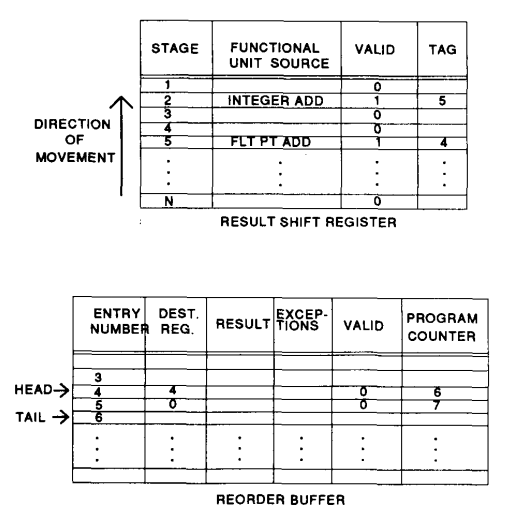
\includegraphics[width=0.5\textwidth]{imagenes/reorder-buffer}
	\caption{Reorder buffer}
	\label{fig:reorder-buffer}
\end{figure}

El buffer contiene un puntero a la entrada que corresponde a la próxima instrucción a ser ejecutada. Cuando dicha entrada contenga información válida, se  chequea si hubo excepciones. Sí no las hubo, se modifican los registros/memoria necesarios y se mueve el puntero a la próxima entrada. Sino, se emite la excepción y se invalidan todas las entradas posteriores.

En algunos casos, la dependencia entre instrucciones requiere el uso de valores que todavía no fueron escritos en los registros. Para conseguirlos es necesario acceder al buffer de reordenamiento, lo que agrega latencia y complejidad a la ejecución.

\paragraph{History Buffer:} Una solución posible es dejar que las instrucciones modifiquen los registros cuando son completadas, pero que se guarden los valores previos en un buffer que permita recuperar estos datos en el caso de una excepción.

En este caso, si ocurre una excepción, se debe recorrer el history buffer para poder recuperar un estado preciso.

\paragraph{Future File:} Otra solución es mantener dos archivos de registros. Uno que se actualice en el orden especificado por el programa (\textbf{Architectural File}). Y otro que se actualiza apenas se completa una instrucción (\textbf{Future File}).

Si ocurre una excepción simplemente se debe mostear el Architecture File para conseguir un estado preciso. Sin embargo, hay que copiarlo al future file para restaurar el estado del sistema.

\paragraph{Checkpointing:} Cuando se predice el resultado de una instrucción de control, se guarda el estado del future file (\textbf{checkpoint}). Si al ejecutarla, la predicción resulta ser errónea entonces solo hay que copiar la información del checkpoint en el future file para recuperar el estado del sistema y comenzar de nuevo en la instrucción correcta.  


\newpage
\part{Procesadores Intel}
\red{A partir de acá resumenes de  los papers. Faltan los que hablan del Intel Core 2.}
\section{Netburst microarchitecture (Pentium 4 \cite{Sager01themicroarchitecture})}
La microarquitectura de este procesador se puede separar en 4 grandes bloques: Front End, Out-of-order engine, Integer and Floating Point Execution Units and the memory subsytem.

\begin{figure}[ht]
	\centering
	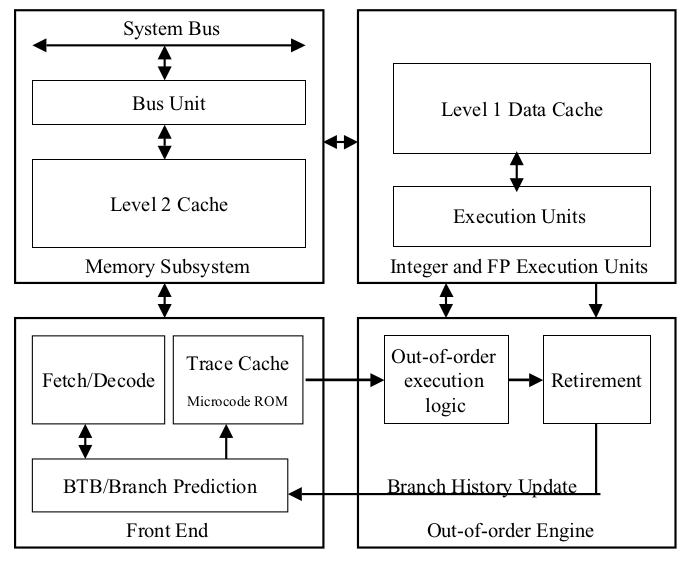
\includegraphics[width=0.35\textwidth]{imagenes/p4-block-architecture}
	\caption{Diagrama básico}
	\label{fig:p4DiagramaBasico}
\end{figure}
\begin{figure}[ht]
	\centering
	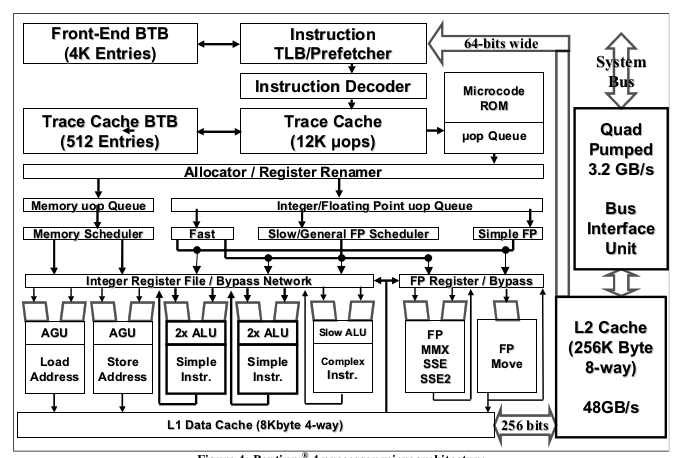
\includegraphics[width=0.8\textwidth]{imagenes/p4-architecture}
	\caption{Architectura del procesador}
	\label{fig:p4DiagramaCompleto}
\end{figure}

\subsection{Front end}
Se dedica al fetcheo y decodificación de instrucciones y la predicción de saltos. Esta compuesto por:
\subsubsection*{Instruction Translation Lookaside Buffer (ITLB)}
Traduce las direcciones lineales del puntero de instrucciones en las direcciones físicas necesarias para acceder a la caché L2. Además, realiza los chequeos de permisos de paginación.

\subsubsection*{Front end Branch Target Buffer}\label{sec::Intel::Netburst::frontEnd::btb}
Fetchea las instrucciones IA-32 que deben ser ejecutadas de la caché L2. El uso de Branch Prediction permite al procesador comenzar a fetchear y ejecutar instrucciones mucho antes de que el outcome de las ramificaciones sea averiguado.
	
Si una rama no se encuentra en el BTB, el hardware de predicciones decide que hacer dependiendo el desplazamiennto de la rama (\textbf{forward} o \textbf{backward}). Backwards branches se asumen Taken y Forward Branches se asumen Not-Taken.

\subsubsection*{IA-32 Instruction Decoder}
Recibe las instrucciones IA-32 desde la caché L2 y las decodifica en primitivas (llamadas micro-operaciones). Una vez decodificadas, si la instrucción consiste en menos de 4 micro-operaciones, entonces es almacenada en la \textbf{Trace Caché}. Sino es enviada a la \textbf{microcode ROM}.

\subsubsection*{Trace Caché} 
Es la caché de instrucciones primaria o de Nivel 1 (\textbf{L1}) donde se guardan ya decodificadas en forma de micro-operaciones. Una vez almacenadas, cada micro-op puede ser usada repetidamene cono si fuese una caché de instrucciones convencional.

Las instrucciones IA-32 tienen un número variable de bits y muchas opciones. La lógica de decodificación necesita tener en cuenta esto y convertirlas en micro-operaciones que la máquina sepa como ejecutar. Esto se hace especialmente difícil cuando se tratan de decodificar varias instrucciones en un único ciclo de reloj de alta frecuencia. Además, cuando la predicción de un branch es errónea, el tiempo de recuperación es mucho más corto si la máquina no tiene que re-decodificarlas para reanudar la ejecución en el lugar correcto.
	
El cacheo de las micro-operaciones permite, a la microarquitectura, evitar el uso decodificador de instrucciones IA-32 durante gran parte de la ejecución.

La caché ensambla las micro-ops en secuencias llamadas trazas (\textbf{traces}) que respetan el orden de ejecución predecido del programa. Esto permite que el target de los branch sean incluidos en la misma linea de traza incluso si estan separados por miles de bytes en el programa. Así, tanto el target como el branch, pueden ser enviados al motor fuera-de-orden al mismo tiempo.

La mayoría de las instrucciones son fetcheadas y ejecutadas desde esta caché. Solo cuando hay un caché miss, la microarquitectura fetchea y decodifica la instrucciones desde la caché \textbf{L2}.

La caché tiene su propio BTB (TBTB) para predecir cual es la próxima micro-operación a ser ejecutada. Esta es más chica que la BTB principal ya que solo debe realizar predicciones sobre el subset de instrucciones presentes en la caché.

\subsubsection*{Microcode ROM}
Esta ROM es usada para instrucciones IA-32 complejas como mover strings y para manejar faults e interrupciones.

Cuando se encuentra una instrucción IA-32 compleja, la Trace Chache la llama y, ésta, emite las micro-operaciones necesarias para ejecutarla. Cuando termina de hacer esto, el control vuelve al Trace Caché.

Las micro-operaciones que provienen de la caché y la microcode ROM son encoladas en un buffer ordenado (\textbf{uop queue}), lo que ayuda a suavizar el flujo de micro-operaciones al Out-Of-Order Engine.

\subsection{Out-of-order engine}
Reordena las instrucciones para que sean ejecutadas apenas todos sus operandos estén listos y se encarga de presentar el estado correcto al front end cuando es necesario modificarlo. Su principal tarea es extraer paralelismo del flujo de instrucciones preservando la semántica de ejecución correcta del programa. Esto lo logra reordenando las micro-operaciones de acuerdo a sus dependencias y las disponibilidad de sus operandos.


\subsubsection*{Allocator (Asignador de recursos)}
El allocator se encarga de distribuir los recursos (entradas del archivo de registros, buffers, ALUs, etc) del sistema entre las micro operaciones que deben ser ejecutadas. Si un recurso no está disponible para alguna de ellas, se pausa la asignación por un ciclo de reloj. Cuando todos los recursos están disponibles, entonces los asigna a las instrucciones correspondientes y las despacha al pipeline para que sean ejecutadas.

A todas las instrucciones les asigna una entrada en el reorder buffer (para mantener un seguimiento del estado en el que se encuentran), el registro donde se guardarán sus y una entrada en alguna de las colas para scheduling.

\subsubsection*{Register Renaming}
El proceso de renombre remueve falsos conflictos causados por múltiples instrucciones independientes que necesitan de un mismo registro. Esto se logra creando varias instancias del mismo registro que indiquen quien las escribió por última vez y el valor adecuado. Ver sección \ref{ilp::superscalars::fetchDecode} 

\subsubsection*{Scheduling de micro-operaciones}
Hay dos colas FIFO, una para operaciones de memoria y otra para el resto. Las colas son atendidas en cualquier orden, lo que permite que la ventana de ejecución fuera de orden sea más grande.

Hay varios schedulers, que se encargan de procesar distintos tipos de instrucciónes. Cada uno de ellos puede determinar cuando una micro-operación está lista para ser ejecutadas (cuando todos sus operandos fueron generados) trackeando sus registros de entrada. Cuando esto sucede, el scheduler la agrega a la cola de ejecución.

El scheduler detecta los flujos de ejecución independientes en una secuencia de micro-operaciones y permite que sean ejecutados paralelamente sin importar su orden general.

Los scedulers, están conectados a distintos puertos de despachos que envían las instrucciones a sus respectivas unidades de ejecución.

\subsection{Integer and Floating Point Excution Units}
Es donde se ejecutan las instrucciones.
Los registros de enteros y los de puntos flotantes se encuentran separados. Cada archivo de registros está conectado a una red que permite enviar resultados completos que todavía no fueron escritos en los registros a las nuevas micro-operaciones.

\subsubsection*{Low Latency Integer ALU}
Está diseñada para optimizar performance manejando los casos más comunes tan rápido como sea posible. Es capaz de completar operaciones en medio ciclo del reloj principal. Aproximadamente el 60-70\% de las micro-operaciones de enteros pasan por ella. Ejecutandolas a la mitad de la latencia del clock principal ayuda a acelerar la ejecución de la mayoría de los programas.

\subsubsection*{Complex Integer Operation}
Los shift, rotaciones multiplicaciones y divisiones tienen una larga latencia (ocupan varios ciclos de reloj), por esta razón son mandados a otros componentes más complejos. 

\subsubsection*{Low Latency Level 1 (L1) Data Cache}
La latencia de las operaciones de lectura es un aspecto clave en la performance del procesador. Esto es especialmente verdad para los programas del IA-32 porque hay un limitado numero de registros en el ISA. Por esta razón, se agrega una pequeña caché de baja latencia que consigue su información desde una caché de segundo nivel. La L2 es más grande, tiene un gran ancho de banda y latencia media.

Con la alta frecuencia y la profundidad del pipeline del pentium 4, el scheduler de micro-operaciones despacha instrucciones más rapido de lo que el load puede ser ejecutado. En la mayoría de los casos, el scheduler asume que hubo en hit en la caché L1. Si la lectura genera un miss entonces habrá, en el pipeline, operaciones dependientes con información errónea que deben volver a ser ejecutadas. Para esto se utiliza un mecanismo conocido como \textbf{replay} que trackea las instrucciones durante su ejecución y, si ocurre el caso mencionado, las detiene e intenta ejecutar nuevamente. 

\subsubsection*{Store-To-Load Forwarding}\label{sec::Intel::NetBurst::FrontEnd::Forwarding}
Los datos son escritos en la caché L1 en el orden programático y solo cuando se puede garantizar que el valor es no-especulativo. Es decir, todas las operaciones anteriores a la isntrucción de almacenamiento deben haber sido completadas antes de que sea commiteado. Debido a la profunidad del pipeline, esto puede tomar varios ciclos de reloj.

A menudo, nuevas instrucciones deben hacer del dato que se está reteniendo y hacerlas esperar hasta que estén en la caché deterioraría el performance del pipeline. Por esta razón, se utiliza un buffer de escrituras pendientes (\textbf{pending store buffer} o \textbf{store forwading buffer}, SFB) que permite que los resultados que todavía no fueron escritos en cache sean utilizados por ellas. Este proceso es llamado \textbf{store-to-load forwarding}.

Cuando una instrucción necesita un dato, en paralelo con el acceso a caché, se reliza una comparación parcial de la dirección con todas las entradas en el SFB. Si hay algun match entonces se carga la información desde el buffer en vez de usar la caché. Se utiliza una comparación parcial para que la latencia del mecanismo sea la misma que la del lookup de la caché.

Mas adelante en el pipeline, un \textbf{Memory Ordering Buffer} debe asegurar que el dato forwardeado provenga de la escritura más reciente. En caso que el forwarding sea incorrecto, entonces la lectura debe ser ejecutada otra vez después de que todos los writes de los que depende hayan sido guardados en caché.

El forwarding puede ser realizado solo cuando se cumplen las siguientes condiciones:
\begin{itemize}
	\item El load utiliza la misma dirección que haya sido completado pero todavía no commiteado en caché (osea que se encuentre en store forwading buffer).
	\item El dato pedido deber ser del mismo tamaño o más chico que el del store pendiente e iniciar en la misma dirección.
\end{itemize}

Si la información pedida por el load se superpone parcialmente con la información del store o necesita hacer uso de más de dos stores pendientes, entonces el forwarding no se permite y  la instrucción debe conseguir su data desde la caché luego de que las operaciones pendientes sean commiteadas.


\subsubsection*{FP/SSE Execution Units}
Es donde se ejecutan las operacion de punto flotante, MMX, SSE y SSE2.
\subsection{Memory Subsysten}
El sistema de memoria, compuesto por una caché L2 y el bus del sistema.

\subsubsection*{Level 2 Instruction and Data Cache}
Contiene las instrucciones que hacen miss en la Trace Cache y la información que produce un miss en la cache L1. Es una caché asociativa de 8 vías y usa un algoritmo write-back para escribir las modificaciones en memoria.

A esta caché se asocia un prefetcher que monitorea los patrones de acceso a memoria y recuerda la historia de los misses para detectar flujos de datos concurrentes y rellenar la caché con información que podría ser utilizada más adelante por el programa. Además, intenta minimizar el prefetching de datos que podrían causar una sobrecarga de la memoria del sistema y provocar el delay de los accesos que el programa realmente necesita.

\subsubsection*{400Mhz System Bus}
Tiene un ancho de banda de 3.2 Gbytes por segundo, esto permite que las aplicaciones realizen data streaming desde la memoria. Tiene un protocolo que divide las transacciones y un pipeline profundo para permitir que el subsistema de memoria atienda varios accesos/escrituras simultáneamente. 

\newpage
\section{Thread Level Paralelism (Procesadores Xenon \cite{marr02threads})}

Tradicionalmente, para mejorar el perfomance, los diseñadores se enfocaban en desarrollar relojes de alta velocidad, ejecución paralela de instrucciones y caches. Sin embargo, en los últimos años, con el desarrollo del internet, se ha visto la necesidad de ejecutar varias tareas simultáneamente. Por esta razón, se han comenzado a desarrollar distintas técnicas de paralelismo a nivel thread (procesos):

\begin{itemize}
	\item \textbf{Chip multiprocessing:}
	 Se utilizan dos procesadores. Cada uno de ellos tiene a su disposición un conjunto completo de recursos de ejecucion y arquitecturales. Pueden o no compartir una caché de primer nivel. Tiene como desventaja que el chip resultante es mas grande y consume más que un chip single-core.
	\item\textbf{Time-slice multithreading:} Un solo procesador ejecuta múltiples threads switcheando entre ellos. El switching se haces después de un determinado período de tiempo o cuando se produce un evento de larga latencia (operaciones que tomen demasiados ciclos de reloj, como lecturas de memoria). La primer opción genera demasiado tiempo muerto que podría ser aprovechado para ejecución de instrucciones, la segunda sirve para aplicaciones de servidores que tienen un gran número de caché misses y ambos threads ejecutan tareas similares. Ninguna de ellas logra superposición optima cuando varias fuentes usan ineficientemente los recursos (branch mispredictions, instrucciones dependientes, etc).
	\item \textbf{Simultaneous multi-threading:} Varios threads pueden ser ejecutados simultaneamente en un solo procesador sin necesidad del switching. Este método es el que mejor aprovecha los recursos del procesador y es el que implementa la arquitectura de Hyper-Threading de Intel.
\end{itemize}

\subsection{Hyper-threading technology architecture}

La tecnología de hyper-threading hace que un procesador físico aparezcan como múltiples procesadores lógicos en la arquitectura. Osea que los programas y los sistemas operativos usarán los procesadores lógicos como si fuesen físicos, luego la microarquitectura se encargará de realizar la distribución de recursos necesarias entre los procesadores físicos.

En chips normales, cada procesador tiene una copia completa del estado de las arquitecturas (registros de proposito general, de control, de interrupciones y algunos de estado de la maquina). 

En hyper-threading, cada procesador físico tiene una copia completas de este estado y un controlador de instrucciones programables (APIC) por cada procesador lógico que contenga.  Las cachés, unidades de ejecución, branch predictors, lógicas de control y buses son compartidas por todos ellos.

\begin{figure}[ht]
	\centering
	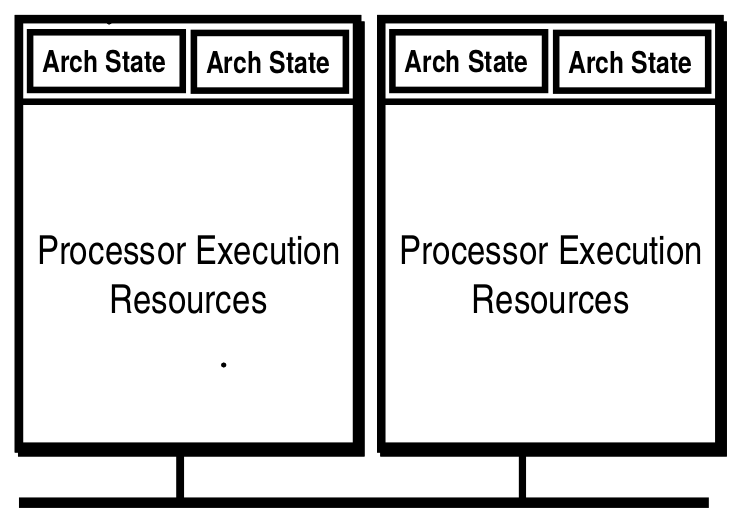
\includegraphics[width=0.5\textwidth]{imagenes/multithreading-procesor}
	\caption{Procesador con tecnología de hyper-threading}
	\label{fig:xenonHyperThreadingTechnology}
\end{figure}

\subsubsection{Front-End}
\paragraph{Execution Trace Cache (TC):}
Por cada procesador lógico, la caché tiene un set de next-instruction-pointers que trackean independientemente el progreso de alguno de los dos threads ejecutandose. Si ambos necesitan accederla al mismo tiempo, el acceso se otorga a uno de ellos y luego al otro en ciclos de reloj alternados.
	
Si uno de los procesadores lógicos está bloqueado (\textit{stalled}) o es incapaz de usar la TC, el otro puede usar la caché completamente (cada ciclo de reloj).

Cada entrada de la caché tiene un tag que indica el thread al que pertenece y es reservada dinámicamente según sea necesario.

\paragraph{Microcode ROM:} Se usan dos punteros para contolar independientemente los flujos si los dos procesadores lógicos están ejecutando instrucciones complejas. Comparten las entradas de la ROM. El acceso es alternado de la misma manera que en la trace caché.

\paragraph{ITLB y Branch Prediction:} Cada procesador lógico tiene su propia ITLB y su propio conjunto de punteros a instrucciones, esto permite trackear el progreso de fetch para cada uno de ellos por separado.

La lógica de fetch a cargo de hacer requests a las caché L2, los arbitra en orden first-come first-served manteniendo reservado un espacio para cada procesador en la cola. De esta manera, ambos procesadores lógicos pueden tener fetches pendientes simultáneamente. 

Una vez fetcheadas, cada procesador lógico tiene su propio conjunto de buffers para retener las instrucciones que deben ser decodificadas.

El \textit{return stack buffer}, que predice la dirección a la que debe retornar una instrucción, es duplicado ya que las predicciones son mejores si se hacen independientemente para cada thread.

Cada procesador lógico tiene un \textit{branch history buffer} local y los dos comparten un buffer global en el que, a cada entrada, se agrega un tag con el ID del procesador al que corresponde.

\paragraph{IA-32 Instruction Decode: } Se comparte este componente. Cuando los dos threads tiene que decodificar instrucciones simultáneamente, la lógica de decodificación alterna el uso de los buffers. En general, varias instrucciones de un mismo procesador son decodificadas antes de pasar al otro.

A pesar de decodificar las instrucciones de cada procesador lógico por separado, se mantiene una copia de todos los estados necesitados para decodificarlas por cada uno de ellos. 

Si solo un procesador necesita usar el decodificador, se le asigna el uso completamente a éste. Las instrucciones decodificadas se escriben en la Trace Caché y son forwardeadas a la cola de micro-operaciones.

\paragraph{Cola de micro operaciones (uop queue):} Está particionada para que cada procesador lógico tenga la mitad de las entradas.

\subsubsection{Out-of-order execution engine}

\paragraph{Allocator:} Cada procesador lógico solo puede usar la mitad de entradas de los buffers principales (de reordenamiento, tracing y secuencialización).

\begin{itemize}
	\item Si ambos procesadores tienen micro-operaciones en la uop queue, el allocator las atendera alternadamente en cada ciclo de reloj.
	\item Si uno de ellos ha alcanzado el límites de recursos que puede usar, le manda una señal para bloquearlo \textit{stall} hasta que libere alguno.
	\item Si la uop queue solo contiene micro-operaciones de uno de los procesadores, el allocator lo atenderá en cada ciclo (manteniendo el limite de asignación de recursos).
\end{itemize}
 
 La límitación de recursos ayuda a la máquina, a reforzar \textbf{fairness} (uso justo) y previene deadlocks. 
 
\paragraph{Register Rename}
Dado que cada procesador lógico debe mantener y traquear su propio estado de arquitectura, hay un register alias table por cada uno. El proceso de renombre se realiza en paralelo a la asignación de recursos (mientras el allocator está trabajando) por lo que la lógica de renombre trabaja sobre las mismas micro-operaciones que el allocator.

Una vez que los dos componentes mencionados terminan de procesar una operación, ésta es ubicada en la cola correspondiente (general o de memoria) a la espera del scheduler.

\paragraph{Instruction Scheduling:} 
La cola general y la de instrucciones de memoria les envian micro-operaciones tan rapido como puedan alternando las instrucciones de ambos procesadores.

Cada scheduler tiene su propia cola de scheduling. Para  asegurar fairness, cada procesador lógico puede tener un limitado número de entradas activas en éstas (este limite es independiente de su tamaño). A parte de eso, al momento de evaluar las micro-operaciones, el scheduler solo se basa en la dependencia de inputs y la disponibilidad de recursos para elegirlas.

\paragraph{Execution units}
Dado que los registros lógicos fueron renombrados a registros físicos en un achivo físico de registros compartidos, para ejecutar las microoperaciones solo es necesario acceder a éste. Por lo que las unidades de ejecución funcionan igual que antes.

Después de la ejecución, las micro-operaciones son enviadas al buffer de reordenamiento que está particionado de tal manera que cada procesador lógico solo pueda la mitad de sus entradas.

\paragraph{Retirement:} Cuando hay micro-operaciónes de ambos procesadores lógicos que deben ser retiradas, se  retiran las instrucciones en orden del programa altarnedamente.

Si un procesador lógico no está listo para retirar ninguna instrucción, entonces se atiende completamente al otro procesador..

Una vez que los almacenamientos han sido retirados, deben ser escritos en la caché L1 del procesador físico. Para esto, se commitea en caché atendiendo alternadamente a cada procesador lógico.

\subsubsection{Subsistema de memoria}

\paragraph{Direction Tranlation Lookaside Buffer (DTLB):} Traduce direcciones a direcciones físicas. Es compartido. Cada entrada incluye el ID del procesador lógico a la que está asignada. Además, cada uno de ellos, tienen reservado un registro para asegurar fairness y progreso al procesar los DTLB misses.

\paragraph{L1, L2 y L3 Data Caches:}
Son cachés asociativas con líneas de 128-bytes. Los dos procesadores lógicos comparten todas sus entradas.

Las caches son ajenas a la lógica de multithreading. Esto puede llegar a potenciales conflictos lo que podría resultar en un deterioro del performance. Sin embargo, tambien existe la posibilidad de que uno de los procesadores pida información que el otro quiera usar. En estos casos, el performance se ve benificiado.

\paragraph{Bus:} Incluye al controlador de interrupciones programables (APIC) local.
La cola de requests y los buffer de espacios son compartidos. Los request al APIC local y los recursos de envío de interrupciones son únicos para cada procesador lógico. Las requests de cada uno de ellos es distinguida con un tag pero no se les da ningun tipo de prioridad.

\subsection{Modos Single-Task y Multi-Task}
\begin{itemize}
	\item \textbf{Multi-Task Mode (MT):} Los dos procesadores lógicos se encuentran activos y los recursos compartidos se dividen como fue descrito anteriormente.
	\item \textbf{Single-Task Mode (ST):} Solo un procesador lógico está activo y los recursos que habían sido particionados en modo multi task son completamentes asignados a éste.
\end{itemize}
\begin{figure}[ht]
	\centering
	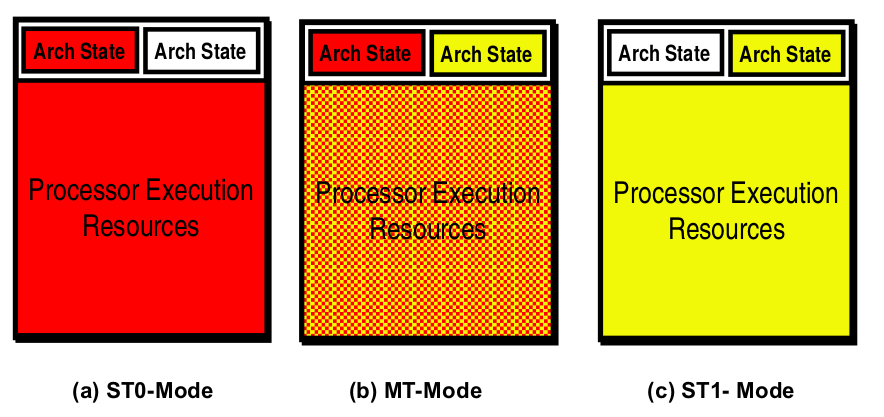
\includegraphics[width=0.75\textwidth]{imagenes/single-multi-task-modes}
	\caption{Asignación de recursos para los distintos modos}
	\label{fig:xenonSingleMultiTaskModes}
\end{figure}
La arquitectura IA-32 tiene una instrucción llamada HALT que para la ejecución de un procesador y le permite entra en modo de bajo consumo. Ésta es una instrucción privilegiada, es decir, solo pueden ejecutarla el sistema operativos y procesos de privilegio 0.

En un procesador con tecnología de hyper-threading, HALT transiciona de modo MT a ST0 o ST1 dependiendo de en que procesador lógico se halla ejecutado la instrucción. Si fue ejecutada por el procesador 0, entonces solo queda activo el 1 y viceversa.

Si se envía una interrupción a un procesador halteado entonces se vuelve a modo MT.

\subsection{Sistemas operativos y aplicaciones}
El sistema operativo se debe encargar de implementar dos optimizaciones para obtener el mejor rendimiento posible.

La primera es usar la instrucción HALT si uno de los procesadores lógicos está activo y el otro no. Un sistema operativo que no use esta optimización hará que el procesador que no se encuentra en uso entre en un idle-loop durante el cual se ejecutaran instrucciones para chequear si hay trabajo para hacer. Este loop puede llegar a consumir una cantidad significante de recursos de ejecución que podrían ser usados por el procesador lógico activo.

La segunda optimización es que, al momento de realizar el scheduling de threads, se los debería mandar a procesadores físicos distintos. Cuando esto ya no sea posible, recién ahí comenzar a usar los procesadores lógicos.

\newpage
\section{Intel Enhanced SpeedStep Technology (Pentium M \cite{Gochman2003TheIP})}

Diseñar un procesador \textit{Mobile} requiere considerar distintso tradeoffs de consumo/performance que no son necesarios en los procesadores tradicionales.

\begin{itemize}
	\item \textbf{Potencia, consumo de energía y temperatura}: Para mantener los transitores en un rango de temperatura de trabajo aceptable, el calor generado tiene que ser disipado de una manera costo-efectiva. Este problema aplica tanto a Mobile como a Desktop, sin embargo, en Mobile, el tamaño y peso de los dispositivos decrementan considerablemente el pico de consumo energético del procesador.

	\item \textbf{Vida de la bateria:} Mientras más alta sea la potencia promedio usada menos es el tiempo durante el que puede operar una batería. Esto limita el consumo de potencia promedio del procesador.
\end{itemize}

\subsection{Power-Awareness Philosophy and strategies}
Se intenta: 
\begin{itemize}
	\item Conseguir un buen balance entre rendimiento y duración de la batería.
	\item Intercambiar rendimiento por energía y viceversa, cuando sea necesario.
\end{itemize}

\paragraph{Más rendimiento vs Mayor duración de la bateria:} Respecto a esto no hicieron nada porque el procesador ya producía menos del 10\% del consumo de energía y no iban a lograr ninguna mejora decente.

\subsubsection{Intercambio entre rendimiento y energía}
 Hay veces en las que implementar un feature que permita ganar performance o ahorrar energía es mejor que simplemente escalar el voltaje/frecuencia de trabajo (método que se usaba en procesadores anteriores). La lógica y componentes necesarios para implementarlas aumenta el consumo de energía pero la ganancia (en tiempo) que generan superan este costo.

Algunas de las features que se agregaron fueron:
\begin{itemize}
	\item\textbf{Reducir el número de instrucciones por tarea:} Se utilizan mejores predictores para disminuir el número de instrucciones mal especuladas lo que reduce el número total de instrucciones procesadas.
	
	\item\textbf{Reducir el número de micro-ops por instrucción:} Atender y ejecutar cada instrucción consume energía. Eliminando micro-operaciones del flujo de ejecución o combinando varias de ellas se reduce el consumo total.
	
	\item\textbf{Reducir el número de switches entre transistores por micro-op:} Procesadores de alto rendimiento  proveen un alto nivel de paralelismo de instrucciones provocando demasiados switches. En algunos casos, se pueden realizar optimizaciones locales (por ejemplo, activar solo la parte que se va a usar de un componente). En otros, se agregan componentes que deciden si una unidad va a estar activa o no en el próximo ciclo y las apaga en caso de que ocurra lo segundo.
	
	\item\textbf{Reducir la cantidad de energía por switch de transistor:} Depende de la cantidad de transistores usados, su tipo, el voltaje de operacion y temperatura. Se utilizan dispositivos de descarga lenta (\textit{low-leakage}) y la tecnología Intel SpeedStep para disminuir los switches y, por lo tanto, el consumo energético. 
\end{itemize}

\subsection{Branch Prediction avanzado}

Se utiliza como base el predictor del Pentium 4. Se le agregan dos componentes adicionales: Un detector de Loops y un predictor de branchs indirectos.

\paragraph{Detector de Loops:} Analiza branches para ver si se comportan como loops. Esto es, si se mueven en una dirección (taken o not-taken) un número fijo de veces intercalando con único movimiento en la dirección opuesta. Cuando este comportamiento es detectado, se crea un conjunto de contadores que permite predecir con toda precisión el comportamiento del programa para iteraciones largas.

\paragraph{Indirect Branchs:} Son generadas por instrucciones de control que, en vez de especificar la dirección a la que hay que saltar, indican donde está guardada esa dirección. Lenguajes como C++ y Java los usan para los switch case.

\paragraph{Indirect Branch Predictor:} Predice basandose en el history buffer. Los targets siempre están ubicados en la tabla de punteros a instrucciones junto con el tipo de branch que las usa. Cuando ocurre una predicción errónea en un indirect branch, el predictor almacena una nueva entrada en la tabla de punteros que corresponde a la entrada del history buffer que apunta a esta instrucción.

Cada branch indirecto puede guardar tantas targets como sea necesario para diferentes patrones de historia global. Esto permite predecir correctamente usando solo la tablas de punteros.

\subsection{Fusión de micro-operaciones}
Una micro-operacion consiste en una única operación y dos operandos fuente. Algunas instrucciones deben ser decodificadas en mas de una micro-operación porque tienen que usar mas de dos operandos, o porque requieren completar una secuencia de operaciones no relacionadas. Esto tiene algunas desventajas:
\begin{itemize}
	\item El gran número de micro-operaciones crea presión en los recursos con  ancho de banda o capacidad limitada.
	
	\item El proceso de decodificación es más complejo que para aquellas instrucciones que se traducen en una única micro-operación.
	
	\item Enviar más micro-operaciones al sistema incrementa la energía requerida para completar una secuencia de instrucciones dada.
\end{itemize}

Con el mecanismo de fusión, el decoder puede fusionar dos micro-operaciones en una. A la micro-operación resultante se le asigna una única entrada en el Reorder Buffer y en el Reservation Station (RS) (cada una de sus entrada puede acomodar tres operandos fuente para soportar este nuevo tipo de operacion). 

El dispatcher trata cada una de ellas como si ocupasen la entrada completa. Ambas micro-operaciones pueden ser emitidas a sus respectivas unidades de ejecución en paralelo. Recién cuando las dos se ejecutaron completamente, pueden ser retiradas como una micro-operacion fusionada.

\begin{figure}[ht]
	\centering
	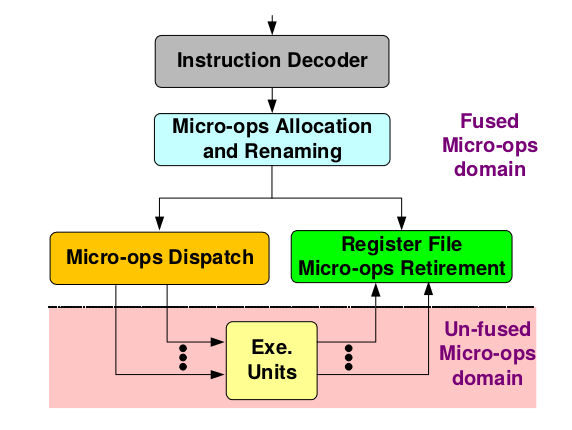
\includegraphics[width=0.75\textwidth]{imagenes/micro-op-fusion}
	\caption{Dominios de fusión de micro-operaciones}
	\label{fig:MicroOpFusion}
\end{figure}

\subsection{Dedicated Stack Engine}
La ISA provee las instrucciones PUSH, POP, CALL y RET que controlan el comportamiento del stack. Además posee el registro ESP (Stack Pointer Register) que es modificado por cada una de estas instrucciones.

En el Pentium M, este efecto es implementado usando lógica dedicada cerca de los decodificadores. La idea es representar el punto de vista del programador ($ESP_P$) en cualquier momento usando un ESP historico ($ESP_O$, que se encuentre en el motor fuera de orden) y un delta ($ESP_D$, offset mantenido en el front-end).

$$ESP_P = ESP_O + ESP_D$$

Cuando una secuencia de pushs o pops es encontrada en el flujo de instrucciones, el hardware dedicado al stack ejecuta las modificaciones en el decoder y actualiza el $ESP_D$ además de modificar el parámetro de dirección para cada una de las micro-operaciones que referencien el stack. De esta manera, la unidad de generación de direcciones puede calcular la locación de memoria correcta.

Los beneficios de esto son:

\begin{itemize}
	\item Las dependencias respecto del ESP son eliminidas dado que $ESP_O$, usado por el scheduler del motor fuera-de-orden, no cambia durante la secuencia de operaciones de stack. Esto nos da la oportunidad de paralizar aún más la ejecución.
	
	\item $ESP_D$ se actualiza usando sumadores especialmente dedicados lo que libera a las unidades de ejecución general para trabajar en otras micro-ops.
	
	\item Actualizar el $ESP_D$ en el front end elimina las micro-ops de actualización de ESP del motor fuera-de-orden. Esto permite ahorrar energía ya que hay menos micro-ops para ejecutar además de que los sumadores dejan de ser usados para operaciones pequeñas.
\end{itemize}

Dado que el motor dedicado del stack vive al principio del pipeline, todos sus calculos son especulativos. Para recuperar un estado preciso en cualquier momento, los valores de $ESP_0$ y $ESP_D$ deben ser recuperados para todas las instrucciones en la maquina. 

El motor fuera-de-orden mantiene el $ESP_0$ como cualquier otro registro de proposito general y una tabla para guardar el $ESP_D$ por cada instrucción en el pipeline.

Cuando el valor arquitectural ($ESP_P$) se necesita dentro del motor, la lógica de decodificación automáticamente inserta una micro-operación que lo calcula. Cuando esto sucede, el $ESP_D$ es reseteado.

\subsection{El bus del Pentium M}
Es un bus con una cola in-order de 8 transacciones. Fue diseñado para sistemas mobile y ambientes uni-procesador.

\paragraph{Sense amplifiers:} Son componentes electrónicos que amplifican las oscilaciones del voltaje para que los valores lógicos (0 o 1) sean adecuadamente reconocibles.

\paragraph{}
Cuando el bus está en modo idle, ahorra energía agresivamente desactivando todos sus \textit{sense amplifiers} por lo que no consumen nada. El procesador debe enviarle una señal (\textbf{DPWR\#} al bus de datos y \textbf{BPRI} al de direcciones) para que éste los active y puedan ser usados. Después de atender todas las transacciones necesarias, vuelve automáticamente a modo idle.

\paragraph{Low Vtt:} Señal para reducir el consumo del bus. Como esto puede conllevar a ciertos problemas de comunicación se implementa un método de compensación para ajustar dinámicamente la potencia de uso durante la ejecución.

\paragraph{PSI:} Señal para reducir el consumo de toda la plataforma.

\subsection{Optimizaciones de bajo nivel}
Otra forma de optimizar consumo, es apagando los clocks o desactivando partes especificas de un componente.

Algunos componentes son capaces de darse cuenta cuando deben entrar en estado idle agregando un poco de lógica, otros no. 

Para el segundo tipo se crearon controles que pueden identificar o predecir sus periodos idle y ordenar, a la unidad, que reduzca su consumo. La lógica de predicción usada por estos controles debe permitir que el componente se active completamente sin niguna penalidad de performance.

\subsection{Tecnología Enhanced Intel Speedstep}\label{sec::intel::enhancedSpeedStep::enhancedSpeedStep}
En generaciones anteriores de procesadores, esta  tecnología cambiaba el modo de operacion del procesador (Lowest Frequency Mode o Highest Frequency Mode) bloqueando su uso durante la transición. Está transición consiste en ir reduciendo o aumentando en pequeños pasos la frecuencia y el voltaje.

La versión Enhanced trata de abordar los siguientes desafíos:
\begin{itemize}
	\item \textbf{Minimizar indisponibilidad del sistema y el procesador:}  Existen ciertas limitaciones físicas del sistema de suministro de energía durante la transición del voltaje que se traduce en un delay en estos componentes (quedan inhabilitados durante este tiempo).
	\item Se debe prevenir la perdida de eventos del sistema como interrupciones y snoops que fueron bloqueados durante la transición.
\end{itemize}

Para resolver el problema se utilizan tres métodos:
\begin{itemize}
	\item \textbf{Cambio por separado del voltaje y la frecuencia:} Se hace en dos etapas. El voltaje se cambia en peqeños pasos incrementales, previniendo ruido en los clocks y permitiendo que el procesador siga ejecutando durante esta transición. 
	
	\begin{figure}[ht]
		\centering
		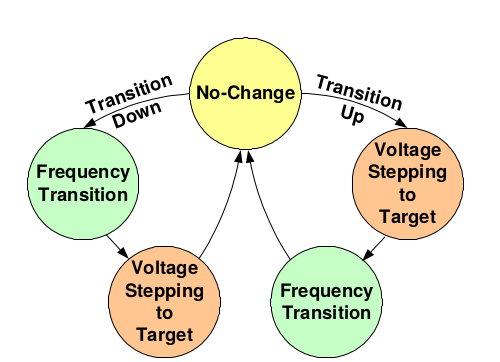
\includegraphics[width=0.5\textwidth]{imagenes/voltage-transitions}
		\caption{Secuencia de transicion de SpeedStep}
		\label{fig:voltageTransitions}
	\end{figure}

\item \textbf{Particionamiento del clock y recuperación:} Se para el clock del core del procesador y el Phase-Locked-Loop (lo que se encarga de transmitir la señal del clock). La lógica de interrupciones y secuenciamiento utilizan el clock del bus (que permanece activo).

\item \textbf{Bloqueo de eventos:}No deben perderse interrupciones, eventos de pin ni pedidos de snoop enviados durante la etapa de transición de frecuencia.

La lógica del SpeedStep samplea todo los eventos de pin cuando el clock del núcleo está parado y son re-enviados al procesador una vez que está disponible.

Los eventos del bus (interrupciones y snoops) son bloqueados usando un protocolo nativo de estos dispotivos que los capturan durante el período de transición de frecuencia.
\end{itemize}

\newpage
\section{Mejoras realizadas al Pentium 4 con la técnología de 90nm \cite{Boggs2004TheMO}}
\subsection{Store-To-Forwarding Enhancement}
Previamente, el forwarding era cancelado cuando las direcciones estaban desalineadas o se forwardeaba un dato incorrecto debido a la comparación parcial de direcicones (Sección \ref{sec::Intel::NetBurst::FrontEnd::Forwarding}).


\paragraph{False forwarding:} Ocurre cuando el SFB detecta un match de dirección parcial entre un load y un store, pero sus direcciónes completas no matchean.

\paragraph{Force Forwarding:} Permite que el Memory Ordering Buffer (MOB) tome control sobre la lógica de comparación parcial del Store Forwading Buffer (SFB).
	
Cuando se necesita hacer un load, el MOB determina su ``verdadera'' dependencia y debe decidir si la decisión del SFB es correcta o si la instrucción debe ser ejecutada otra vez. Si el chequeo de dependencia falla entonces puede corregir la logica del buffer de dos maneras:
	\begin{itemize}
		\item Forzando el forwardeo de la entrada correcta y rotando la data si es necesario (en caso de que el dato se encuentre desalineado).
		\item Desactivando el forwarding si la dependencia no se encuentra en el SFB.
	\end{itemize}
\subsection{Front End}
\subsubsection{Branch Predictor}
Previamente, cuando un branch no se encontraba en el branch target buffer (BTB), si era una rama que saltaba hacia atras (Backward branch) se tomaba como \textit{taken} y si realizaba un salto hacia adelante (forward branch) no
 (Seccion \ref{sec::Intel::Netburst::frontEnd::btb}). Si bien este algoritmo nos permite predecir correctamente cuando el backwards branch es de un loop, no siempre pertenece a uno.

Algunas mejoras en el predictor estático:
\begin{itemize}
	\item Existe un threshold para la distancia entre un backwards branch y su target: Si el BTB no tiene ninguna predicción para una rama de este tipo y la distancia a su target es menor al threshold, entonce predice \textit{taken} sino predice \textit{not-taken}.
	\item Hay branches con ciertas condiciones que, muchas veces, no son tomadas sin importar las dirección ni la distancia. Como estas condiciones no son comunes en loops, se predicen \textit{not-taken}.
\end{itemize}

Al predictor dinámico, se le agrego el Indirect Branch Predictor implementado para el Pentium M para reducir predicciones erróneas.

\subsubsection{Detección de dependencias extras}
En vez de mover un cero a un registro, una técnica común para resetarlo, es usar la instrucción \texttt{xor} consigo mismo. Esta técnica es preferida porque el código escrito es mucho más pequeño.

En una máquina fuera-de-orden, esta extra dependencia puede resultar en perdida de rendimiento. Previos procesadores remueven esta dependencia en el registro fuente dado que el resultado será siempre el mismo sin importar que valor se encuentre en él. Como se agregaron nuevas instrucciones (SSE2) que pueden ser usadas de la misma manera, se agregó lógica para que también sean reconocidas.

\subsubsection{Trace Caché}
Se aumentó su tamaño y puede codificar mas tipos de micro-ops que en previos procesadores. Si una instrucción usa una micro-ops que no puede ser codificada, entonces debe ser secuenciada en la Microcode ROM. Esta mejora permite un mayo ancho de banda de micro-operaciones desde el front end hacia el motor de ejecución fuera de orden ya que remueve varias transciciones al ROM.

\subsubsection{Unidades de ejecución}
\begin{itemize}
\item Se agrega un shifter a una de las ALUs. Esto permite ejecutar estas operaciones  sin necesidad de utilizar recursos que deberían estar destinados a instrucciones complejas de enteros (como se hacia en previos procesadores).

\item Previamente, las multiplicaciones de enteros se ejecutaban en los multiplicadores de puntos flotantes. Esto generaba latencia porque se debían mover los operandos a la zona de punto flotante y después devolverlos a la de enteros. Ahora, hay un multiplicador de enteros especializados que evita esto.

\item El tamaño de la caché L1 aumenta considerablemente su tamaño y el tamaño de la comparación de direcciónes parciales. Esto reduce el número de casos de falso aliasing.

\item Los schedulers dedicados a instrucciones x87/SSE/SSE2/SSE3 aumentan su tamaño, lo que permite que aumente la ventana de oportunidad para encontrar paralelismo en algoritmos multimedia. 

\item Se aumenta el tamaño de todas las colas que alimentan a los schedulers por lo que se pueden bufferear más micro-operaciones antes de que el allocator entre en modo \textit{stall}.

\item Se agrega un predictor que indica si es muy probable que una micro-op de lectura reciba data forwardeada y, si es así, desde que entrada. Dada esta información, el scheduler de loads la retiene hasta que la instrucción de almacenamiento de la que depende sea puesta en la cola de ejecución. De esta forma, se reduce la latencia introducida cuando se debe re-ejecutar una instrucción de lectura fallida.
\end{itemize}

\subsection{Sistema de memoria}\label{secc::intel::90um::memoria}
\paragraph{Cachés:} Se incrementan el tamaño de las cachés para reducir el tiempo que se gasta esperando a que la DRAM devuelva información.

\paragraph{Page Table Walk:} Se recorre la tabla de paginación del sistema para ver si existe un mapeo de alguna dirección especifica.

\paragraph{Software Prefetching:} El programador puede insertar instrucciones de prefetch para traer data a la cache antes de lo necesario. En las versiones previas, estas instrucciones traian datos desde la DRAM hasta la cache L2 para no contaminar la cache L1.

Ahora, se agrega un mecanimos que permite a la instrucción iniciar un page table walk y rellenar al data translation lookaside buffer en caso de que el prefetch se haga sobre una página no cacheada.

\paragraph{Hardware Prefetching:} Un dispositivo detecta flujo de datos e intenta predecir que información va a ser usada a continuación. Este método es superior al software prefecthing ya que no requiere ningún esfuerzo por parte del programador y puede mejorar el rendimiento en código que no tiene instrucciones de prefetch.

\paragraph{Buses:} Se ensanchan los buses y se agregan buffers lo que permite tener una mayor cantidad de lecturas y escrituras simultáneas.

\subsection{Hyper-Threading Technology}
Se resuelven dos cuellos de botellas, que antes no habían sido tenidos en cuenta porque procesadores single-threaded no generaban problemas:

\begin{itemize}
	\item Antes, el procesador solo podía realizar un único page walk o atender un acceso de memoria. En multi-threading esto puede generar un problema por lo que ahora pueden ocurrir simultáneamente una o más veces cada operación.
	\item El esquema de indexación parcial usado para la cache L1 genera conflictos cuando el patrón de acceso de cada procesador lógico matchean al mismo tag parcial incluso si están accediendo a regiones separadas de la memoria física. Esto causa contención en la caché, lo que reduce el hit rate.
	
	Para disminuir la probabilidad de que esto ocurra, por cada procesador lógico, se agrega al tag parcial un bit de contexto. Este bit es seteado o reseteado dinámicamente dependiendo de la inicilización de la estructura de la tabla de paginación de cada procesador. 
	
	Si dos procesadores lógicos intentan compartir el mismo directorio base en la memoria física, el bit de contexto de cada uno de ellos es seteado al mismo valor. Esto les permite compartir las entradas de la caché L1.
	
	Si las direcciones bases del directorio de páginas es diferente entonces es probable que estén trabajando en regiones físicamente separadas. En este caso, los bits de contexto se setean en valores distintos y la cache no se comparte.
\end{itemize}

\newpage
\section{Chip Multi-Processor (Intel Core Duo \cite{gochman2006ICD})}
La tecnología core multi-procesor, a diferencia de predecesores, incluye dos multiprocesadores físicos dentro de un mismo núcleo. 

La tecnología Intel Core Duo se implementó con el objetivo de crear un procesador que sea adecuado para todas las plataformas mobiles (celulares, notebooks, datases, impresoras, etc). se basa en dos microprocesadores Pentium M mejorados que fueron integrados y comparten un caché L2. Con el fin de satisfacer las demandas de rendimiento y consumo se tomaron las siguientes decisiones:

\subsection{Mejoras de rendimiento implementadas}
\begin{itemize}
	\item Mientras que la microarquitectura SSE es de 128 bits de ancho, la del Pentium M es de 64. En estos procesadores, cada instrucción SSE se parte en pares de micro-operaciones de 64 bits lo que implica un cuello de botella en el front end del pipeline durante la etapa de decodificación.  
	
	Una máquina más ancha produciría mas calor e impactaría significativamente en el diseño térmico del sistema y la duración de la batería. Dado que el Pentium M fue diseñado principalmente para mobilidad, se decidió mantener la arquitectura del mismo tamaño y tratar de diluir el problema. Para esto, se introdujo un nuevo mecanismo que permite \textit{laminar}\footnote{El paper no dice que significa laminar pero da a entender que es algo parecido a la fusión} pares de micro-operaciones similares. En cierto punto del pipeline, el flujo de micro-operaciones laminadas es delaminado para ejecutar las micro-operaciones originales. 
	
	Este cambio no solo mejora el rendimiento de las operaciones vectoriales sino que ahorran energía dado que puede ser desactivado cuando el buffer se llena hasta cierto punto.
	
	\item Otro cuello de botella descubierto, fue en el  Floating Point Control Word (FPCW, un componente que controla la precisión de las operaciones de punto flotante). Antes, se consideraba ``constante'' durante la ejecución de un programa, pero en algunos programas se le cambiaba el modo antes de realizar ciertas operaciones. 
	
	Cada una de estas manipulaciones provoca un \textit{stall} en el pipeline. Por esta razón, se introdujo un nuevo mecanismo de renombre para que 4 versiones distintas de este registro puedan coexistir durante la ejecución sin interrumpir el pipeline.
	
	\item Antes, la división se realizaba iterando un número máximo (fijo) de iteraciones, lo que producía largas latencias. En esta versión del procesador, se agregó lógica que calcula el número de iteraciones requeridos para lograr la operación. De esta forma, una vez ejecutada la cantidad de iteraciones requeridas, la división devuelve el resultado.
	
	\item Se agrega un prefetcher de instrucciones a la caché L2 (Ver sección \ref{secc::intel::90um::memoria})

\end{itemize}
\subsection{Estructura general del procesador}
Los procesadores Intel Core Duo utilizan un arquitectura de caché compartida para maximizar el rendimiento de las aplicaciones single y multi-threaded.

\begin{figure}[ht]
	\centering
	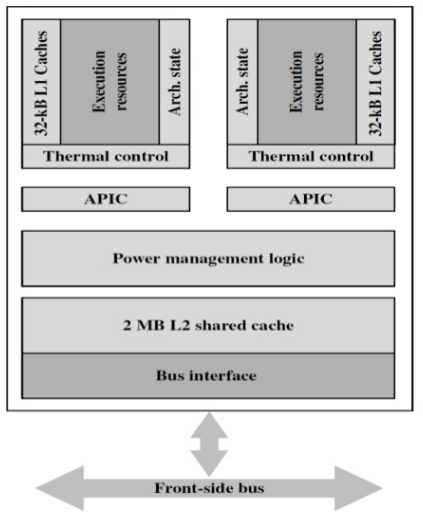
\includegraphics[width=0.375\textwidth]{imagenes/core-duo-block-diagram}
	\caption{Estructura general del Intel Core Duo}
	\label{fig:intelCoreDuoStructure}
\end{figure}

\begin{itemize}
	\item Cada core tiene su propio APIC. Se presentan al sistema operativo como dos procesadores lógicos separadoss.
	\item Cada core tiene su propia unidad de control de temperatura.
	\item El sistema combina control de consumo por cada core y para todo el chip en general.
\end{itemize}

\subsection{Control de consumo energético}
Para disminuir la perdida de energía (cosumo estático), se utilizan dos técnicas: Enhanced Sleep State Control y Dynamic Intel Smart Cache Sizing. Para controlar consumo de energía activa: Se utiliza una técnica basada en Intel SpeedStep technology (Sección \ref{sec::intel::enhancedSpeedStep::enhancedSpeedStep}).

\subsubsection{Leakage power consumption}
\paragraph{} Agregar un segundo core en el chip, demanda una mejora en los estados de consumo del sistema para evitar que se desperdicie energía cuando alguno de los cores no está activo. Se encuentran dos problemas: (1) Utilizar un único circuito de consumo, nos fuerza a correr todos los cores con el mismo voltaje y la misma frequencia, y (2) el chip-set y el OS ven ambos cores como una entidad única con un único estado en cada momento. Por esto, el procesador Intel Core Duo implementa el sistema de estados como dos vistas separadas, internamente cada core maneja sus estados independientemente (per-core power state) y, externamente, el sistema ve un estado de consumo único sincronizado.

Hay cinco estados posibles:

\begin{itemize}
	\item \textbf{C0 - Active (per-core):} Power state is assumed to be in running mode.
	\item \textbf{C1 - Auto halt (per-core):} When the core has nothing to do, the OS issues a halt command that shut off the core clock.
	\item \textbf{C2 - Stop Clock (per-core):} Core and bus clocks are off
	\item \textbf{C3 - Deep sleep (per-core):} Clock generator if off;
	\item \textbf{C4 - Deeper Sleep:} Whole system voltage is reduced. Since the cores are connected to the same power plane, this must be done in coordination between the two cores.
	\item \textbf{DC4 - Deeper C4:}	Further reduce voltage.
\end{itemize}

While being in a sleep state, the system still consumes static power (leakage). In Intel Core Duo Technology, we implement an advanced algorithm that tries to anticipate the effective cache memory footprint that the system need when moving from a deep sleep state to an active mode. The new mechanism keeps only the minimum cache memory size needed active, and it uses special circuit techniques to keep de rest of the cache memory in a state that consumes only a minimal amount of leakage power.

\subsubsection{Active power consumption}
In order to control the active power consumption, Intel Core Duo Technology uses Intel SpeedStep technology. When a set of working points is defined, each one has a different frequency and voltage and so different power consumption. The system can define at what working point it works in order to strike balance between the performance needs and the dynamic power consumption. This is usually done via the OS, using the ACPIs.

\subsection{Thermal Design Point}
In the previous Pentium M processor, a single analog thermal diode was used to measure die temperature. Thermal diode cannot be located at the hottest spot of the die and therefore some offset was applied to keep the CPU within specifications. For these system it was sufficient, since the die had a single hot spot. In the Intel Core Duo processor, there are several hot spots that change position as a function of the combined workload of both cores.

The use of a digital thermometer allows tighter thermal control functions, allowing higher performance in the same form factor. The improved capability also allows us to achieve better ergonomic systems that do not get to hot, can operate more quietly, and are more reliable.

The thermal measurement function provides interfaces to power-management software such as the industry standard ACPI. Each core can be defined as an independient thermal zone, or a single thermal zone for the entire chip. The maximum temperature for each thermal zone is reported separately via dedicated registers that can be polled by the software.

Intel Core Duo technology implemented a dual-core power monitor capability. It continuously tracks the die temperature. If the temperature reaches de maximum allowed value, a throttle mechanism is initiated. Throttling starts with the more efficient dynamic voltage scaling policy and if not sufficient, the power monitor algorithm continues lowering the frequency. If an extreme cooling malfunctions occurs, an Out of Spec notification will be initiated, requesting a controlled complete shutdown.

\subsection{Platfrom Power Managment}
Inter Core Duo processor technology closely interacts with other components on the platform. One such component is the Voltage Regulator (VR).

The CPU has internal knowledge of the activity demand and it communicates a request to go to higher power early enough for the VR to get ready for the increased demand.

\subsection{Intel Core Solo Processor}
In order to fit into very limited thermal constraints and power consumption, the Intel Core Duo processor has a derivative that contains a single core only. This can be achieved:

\begin{itemize}
	\item \textbf{by user or OS decision: }The system will keep the second core idle at CC4 state. Each time an interrupt is received or a broadcast IPI is sent, this core may need to wake up and go immediately back to sleep state, consuming small amounts of dynamic power.
	\item \textbf{by a BIOS option:} The system does not recognize the other core and so it is kept in CC4 state all the time, consumming no dynamic power at all.
	\item \textbf{Total disconnection:} The disadvantage of the two methods described above is that the core still consumes static power. In order to avoid this and reduce the power consumption of the core even further, Intel introduces the single-core version of the Inter Core Duo Technology, called Intel Core Solo Processor, which disconnects the non-active core from the power grid.
\end{itemize}

\newpage
\section{Chip Multi Procesor (Intel Core Duo \cite{Mendelson:2006:CIS}): Known Performance issues}

\subsection{MESI Protocol Modification}
Intel Core Duo processor implements the same MESI protocol as in all other Pentum M processors.

In order to improve performance, we optimized the protocol for faster communication between the cores, particularly when the data exist in the L2 cache.

When a core issues an \textbf{RFO} (Request For Ownership), if the line is shared only by the other cache within CMP die, we can resolve the RFO internally very fast, without going to the external bus at all. Only if the line is shared with another agent on the external bus do we need to issue the RFO externally.

In the case of a multi-package system, the number of coherence messages over the external bus is smaller than in similar DP or MP systems, since much of the communication is being resolved internally.

\subsection{Shared vs Split Cache}
Recently, different architectures use a split last-level cache in order to achieve a fast time-to-market of a dual-core system. Clear downsides of this solution are as follows:
\begin{enumerate}
	\item Cache coherent-related events that need to be served over the File System Buss, such as RFO or invalidation signals, greatly impact performance and power.
	\item An ST application cannot take full advantage of the entire cache.
\end{enumerate}

The hard partitioned cache may prevent one application from significantly reducing the amount of cache memory available to an application running on the other core.

\subsubsection{False Sharing}
False sharing happens when two or more threads access different address ranges on the same cache line simultaneously. This causes the cache line to be in the first level cache of the two cores.

False sharing causes a severe performance penalty if one or more threads writes to the shared cache line. This causes invalidation of the cache line at the L1 cache of the other core. As a ressult, the next time that the other core accesses the cache line in question it will have to transfer it from the core that wrote it earlier through the bus, thereby incurring a mayor latency penalty.

\subsubsection{Parallelizing code thata use great amount of data}
When parallelizing code sections that use data sets exceeding the L2 cache and/or bus bandwith, if one of the threads is using the L2 cache and/or bus, then it is expected to get the maximum possible speedup when the other thread running on the other core does not interrupt its progress. However, if the two threads use the second-level cache there may be performance degradation if one of the following condition is true:
\begin{itemize}
	\item Their combined data set is greater than the L2 cache size.
	\item Their combined bus usage is greater than bus capacity.
	\item They both have extensive access to the same set in the L2 cache, and at least one of the threads writes to this cache line.
\end{itemize}   %%  Y especificaciones de memoria y otras cosas de importancia para furfaro.

\newpage

\part*{Bibliografía}
\nocite{*}
\printbibliography[keyword=intro,title={Introduccion}]
\printbibliography[keyword=ilp,title={Instruction Level Paralellism}]
\printbibliography[keyword=memory,title={Jerarquías de memoria}]
\printbibliography[keyword=intel,title={Procesadores Intel}]
\end{document}

